\documentclass[xcolor={dvipsnames}]{beamer}
\usepackage{color, colortbl}
\usepackage[ngerman,english]{babel}
\usepackage[T1]{fontenc}
\usepackage{lmodern}
\usepackage[compatibility=false]{caption}
\usepackage{subcaption}
\usepackage{tikz}
\usepackage{textgreek}
\usepackage{tabularx}
\usepackage{booktabs}
\usepackage{xspace,multicol}
\usepackage{siunitx}
\usepackage{appendixnumberbeamer}
\usepackage[absolute,overlay]{textpos} %for positioning the logos where I want


\usepackage{animate}
\usepackage{multimedia}
\usepackage{fixltx2e}
\usepackage{multicol}
\usepackage{multirow}
\usepackage{comment}
\DeclareSIUnit\year{yr}
\DeclareSIUnit\micron{\micro\metre}
\DeclareSIUnit\mrad{\milli\rad}
\DeclareSIUnit\gauss{G}
\DeclareSIUnit\nb{\nano\barn}
\DeclareSIUnit\pb{\pico\barn}
\DeclareSIUnit\fb{\femto\barn}

\newcommand{\electron}{e$^-$\xspace}
\newcommand{\positron}{e$^+$\xspace}
\newcommand{\murm}{%
  \ifmmode
    \mathchoice
        {\hbox{\normalsize\textmu}}
        {\hbox{\normalsize\textmu}}
        {\hbox{\scriptsize\textmu}}
        {\hbox{\tiny\textmu}}%
  \else
    \textmu
  \fi
}

\mode<presentation>
{
  \usetheme{CambridgeUS}     
  \usecolortheme{lily} 
  \definecolor{beamer@violet}{rgb}{0.5,0.3,0.5} % changed this
  \setbeamercolor{structure}{fg=beamer@violet!70!cyan}
  \setbeamercolor{palette primary}{fg=black, bg=gray!30!white!50!cyan!20!}
  \setbeamercolor{palette secondary}{fg=black, bg=gray!30!white!30!cyan!40!}
  \setbeamercolor*{palette tertiary}{bg=gray!20!white!20!cyan!60!}
  
  \setbeamercolor{frametitle}{fg=cyan!60!white!40!,bg=cyan!80!black}
  \setbeamercolor{title}{fg=cyan!80!black}
  \setbeamercolor{normal text}{fg=black,bg=white}
  \setbeamercolor{alerted text}{fg=beamer@violet}
  \setbeamercolor{example text}{fg=beamer@violet!70!cyan}
  
  \usefonttheme{structureitalicserif} 
  \setbeamertemplate{navigation symbols}{}
  \setbeamertemplate{caption}[numbered]
}
\newcommand{\sidlogo}{
  \setlength{\TPHorizModule}{1pt}
  \setlength{\TPVertModule}{1pt}
   % textblock{}{x,y}: pos(x) = rightUpperCorner + (x * \TPHorizModule), pos(y) = leftUpperCorner - (y * \TPVertModule)
  \begin{textblock}{1}(323,12)
   \includegraphics[width=40pt,height=26pt]{figures/SiD.jpeg}
  \end{textblock}
  } 
\newcommand{\ilclogo}{
  \setlength{\TPHorizModule}{1pt}
  \setlength{\TPVertModule}{1pt}
   % textblock{}{x,y}: pos(x) = rightUpperCorner + (x * \TPHorizModule), pos(y) = leftUpperCorner - (y * \TPVertModule)
  \begin{textblock}{1}(323,12)
   \includegraphics[width=40pt,height=26pt]{figures/ILC.jpeg}
  \end{textblock}
} 
\newcommand{\flukalogo}{
  \setlength{\TPHorizModule}{1pt}
  \setlength{\TPVertModule}{1pt}
   % textblock{}{x,y}: pos(x) = rightUpperCorner + (x * \TPHorizModule), pos(y) = leftUpperCorner - (y * \TPVertModule)
  \begin{textblock}{1}(315,12)
   \includegraphics[width=60pt,height=26pt]{figures/fluka_logo.png}
  \end{textblock}
} 

\title[ILC backgrounds \& SiD Occupancy]{\textbf{\alert{Mini-Workshop on ILC Infrastructure and CFS for Physics and Detectors} \\ \vspace*{0.3cm} \LARGE  Update \& Summary of \\Background \& SiD Occupancy Studies}}
\author{\textbf{Anne Sch\"utz}}
\institute{\textbf{DESY}}
\date{\textbf{23. February 2018}}

\titlegraphic{\includegraphics[height=1.0cm]{figures/ILC.jpeg}\hspace*{6cm}~%
   \includegraphics[height=1.2cm]{figures/DESY_Logo.png}
}

\begin{document}

{
\usebackgroundtemplate{
 \tikz\node[opacity=0.1]{\includegraphics[width=\paperwidth]{figures/Iwatecomics.jpg}};
 % \tikz\node[opacity=0.2]{\centering\includegraphics[height=\paperheight]{figures/Iwatecomics.jpg}};
 }
\begin{frame}
  \titlepage
\end{frame}
}
\setcounter{tocdepth}{2}
\begin{frame}{Table of contents}
  \tableofcontents
\end{frame}

%---------------------------------------------------------------------------------------------------------

\section{Pair background studies for the new ILC250 schemes}
\begin{frame}
 \begin{center}
  {\LARGE Pair background studies for the ILC250 schemes}
 \end{center}
\end{frame}
\begin{frame}{ILC250 Beam Parameter Sets}
The TDR beam parameters were changed in order to increase the luminosity of the ILC250 stage.
 \begin{table}
\centering
\begin{tabularx}{0.55\textwidth}{llll}
\hline\hline
\textbf{Set}  & \textbf{$\epsilon_x$ [\murm m]} & \textbf{$\beta_x$ [mm]} & \textbf{$\beta_y$ [mm]}\\
\hline
\cline{1-4}
\hline
 TDR & 10 & 13.0 & 0.41\\
 (A) & 5 & 13.0 & 0.41\\
 (B) & 5 & 9.19 & 0.41\\
 (C) & 5 & 9.19 & 0.58\\
\hline\hline
\end{tabularx}
\end{table}
{(\small The table only lists the parameters that are to be changed with respect to the original ILC250 parameters given in the Technical Design Report (TDR)~\cite[p. 11]{TDR1}.)}\\
\vspace*{0.5cm}
\alert{Reduced emittance leads to stronger beam-beam interactions, and therefore to increased \positron \electron pair background.}
\end{frame}

\setcounter{tocdepth}{3}
\AtBeginSubsection[] {
  \begin{frame}<beamer>
     \tableofcontents[currentsection,
     currentsubsection,
     %hideothersubsections,
     subsectionstyle=show/shaded/hide,
     subsubsectionstyle=show/show/hide]
  \end{frame}
}

\subsection{Pair background envelopes}
\begin{frame}{Pair background density in a 5\,T solenoid field}
 \begin{figure}
\centering
\begin{subfigure}[t]{0.35\textwidth}
\centering
\includegraphics[width=\textwidth]{ILC250_figures/Helix_tracks_xz_100bunches_250GeV_5T_DanielJeans-1.jpg}
\caption{ILC250 set (TDR)}
\end{subfigure}
\hspace*{0.1cm}
\begin{subfigure}[t]{0.35\textwidth}
\centering
\includegraphics[width=\textwidth]{ILC250_figures/Helix_tracks_xz_80bunches_250GeV_5T_Reduced_Emittance_x-1.jpg}
\caption{ILC250 set (A)}
\end{subfigure}
\\
\begin{subfigure}[t]{0.35\textwidth}
\centering
\includegraphics[width=\textwidth]{ILC250_figures/Helix_tracks_xz_50bunches_250GeV_5T_Reduced_Emittance_x_Reduced_Beta_x-1.jpg}
\caption{ILC250 set (B)}
\end{subfigure}
\hspace*{0.1cm}
\begin{subfigure}[t]{0.35\textwidth}
\centering
\includegraphics[width=\textwidth]{ILC250_figures/Helix_tracks_xz_50bunches_250GeV_5T_Reduced_Emittance_x_Reduced_Beta_x_Increased_Beta_y-1.jpg}
\caption{ILC250 set (C)}
\end{subfigure}
\caption{Pair background density for the different ILC250 beam parameter sets.
The beam pipe is represented by the red solid lines.}
\label{fig:Envelopes}
\end{figure}

\end{frame}

\begin{frame}{Projection of the pair background density along x}
\begin{center}
 \includegraphics[width=0.72\textwidth]{ILC250_figures/HelixEnvelope_Projection_Comparison_250GeV_parametersets_NEWSETNAMES.png}
\end{center}
The envelopes are in all schemes well contained within the beam pipe. Less than 10 particles per bunch crossing are to be expected outside the beam pipe.
\end{frame}

\subsection{SiD Occupancy}
\begin{frame}{SiD Vertex Detector Occupancy}
 \begin{figure}
\centering
\begin{subfigure}[t]{0.48\textwidth}
\centering
\includegraphics[width=\textwidth]{ILC250_figures/Occupancy_Comparison_All_layers_wrt__cells_ILC250_ALL_SETS_6Sep2017_NEWSETNAMES.png}
\caption{All layers}
\end{subfigure}
\hspace*{0.2cm}
\begin{subfigure}[t]{0.48\textwidth}
\centering
 \includegraphics[width=\textwidth]{ILC250_figures/Occupancy_Comparison_Layer_0_numcells_ILC250_ALL_SETS_6Sep2017_NEWSETNAMES.png}
 \caption{Innermost layer}
\end{subfigure}
\end{figure}
\alert{Normalized Occupancy}: Number of cells containing a certain amount of hits, normalized by the total number of cells of the vertex detector.\\
The occupancy in layer 0 for the new sets is significantly increased with respect to the TDR scheme.
\end{frame}


\subsection{Conclusion}
\begin{frame}{Conclusion}
\begin{itemize}
 \item The SiD vertex detector occupancies for the beam parameter sets (A, B, and C), which contain changes wrt the TDR parameters, are increased by a factor of $\sim$ 2-6.
 \item For all schemes, the \alert{occupancy does not exceed $\sim10^{-4}$ (limit of acceptance)}.
 \item Even \alert{in the innermost layer}, for which the change in occupancy is the highest, the \alert{occupancy for the new parameter set A is below the critical limit}.
\end{itemize}
\textit{Conclusion:}
\begin{itemize}
\item \alert{SiD is confident that the rise in occupancy can be accommodated in the design of the pixel detector, and has welcomed CR-0016.}
\end{itemize}
\end{frame}

%----------------------------------------------------------------------------------
\AtBeginSection[] {
  \begin{frame}<beamer>
     \tableofcontents[currentsection,
     currentsubsection,
     %hideothersubsections,
     subsectionstyle=show/shaded/hide,
     subsubsectionstyle=show/show/hide]
  \end{frame}
}

\section{Muons from the muon spoilers}

\begin{frame}{BDS tunnel layout}
\ilclogo
\begin{center}
\includegraphics[height=0.65\textheight]{muons_figures/BDS_electron_tunnel.pdf}
\end{center}
\end{frame}

\begin{frame}{Muon spoiler scenarios}
\ilclogo
There are two spoiler scenarios under discussion:
\begin{itemize}
 \item \textbf{5 Spoilers}
 \item \textbf{5 Spoilers + Wall}
\end{itemize}

\begin{columns}[b]
 \begin{column}{0.8\textwidth}
 \flushright
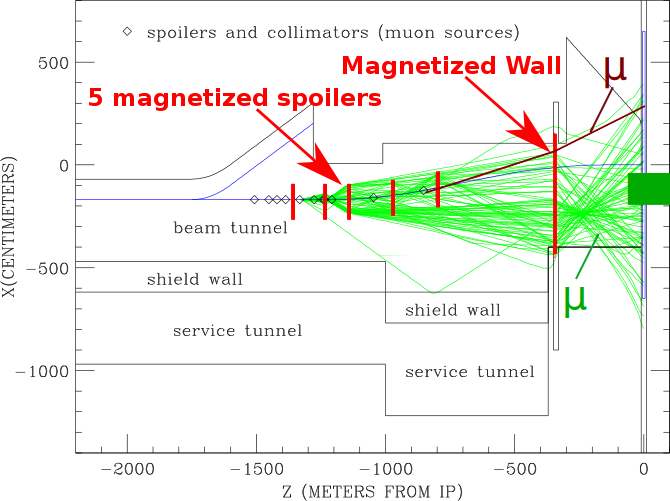
\includegraphics[height=0.67\textheight]{muons_figures/BDS_Tunnel_Spoilers+Wall.png}
\end{column}
 \begin{column}{0.2\textwidth}
 \flushleft
e\textsuperscript{-} beam line
\vspace*{0.55cm}
\end{column}
\end{columns}
\end{frame}

\begin{frame}{5 donut spoilers}
\ilclogo
\textbf{The donut spoilers} are designed as follows:
\begin{itemize}
 \item \SI{70}{\centi\meter} radius
 \item \SI{5}{\meter} long
 \item Magnetized iron with a field of $\sim$10-\SI{19}{\kilo\gauss}
 \item 5 locations (before IP):
 \begin{itemize}
  \item 802.5m
  \item 975.5m
  \item 1145.5m
  \item 1234.5m
  \item 1358.5m
 \end{itemize}

\end{itemize}
\begin{center}
\includegraphics[height=0.3\textheight]{muons_figures/Spoiler.png}
\end{center}
\end{frame}

\begin{frame}{5 donut spoilers + wall}
\ilclogo
\textbf{The iron wall} would completely fill up the tunnel:
\begin{itemize}
 \item \SI{5}{m} x \SI{5}{m}, \SI{5}{m} long
 \item Magnetized with a field of $\sim$\SI{16}{kG}
 \item Located $\sim$\SI{400}{m} away from the IP
 \item Would cost $\sim$ \$3 million
\end{itemize}
\begin{center}
\includegraphics[height=0.7\textheight]{muons_figures/Muon_wall.pdf}
\end{center}
\end{frame}


\subsection{MUCARLO simulation}
\begin{frame}{MUCARLO simulation overview}
\ilclogo

\begin{columns}
 \begin{column}{0.7\textwidth}
  \begin{itemize}
\item BDS backgrounds with muon collimation system modelled with MUCARLO [Lewis Keller, SLAC] and Geant4 [Glen White, SLAC]
\item Using TDR baseline machine parameters for the ILC500 \alert{\& new beam parameters for the ILC250 stage}
\item Muon production processes:
\begin{itemize}
\item Predominantly: Bethe-Heitler process:\\ \textgamma + Z $\rightarrow$ Z' + \textmu$^+$\textmu$^-$
\item Few \% level: direct annihilation of positrons with atomic electrons: e$^+$e$^-$ $\rightarrow$ \textmu$^+$\textmu$^-$
\end{itemize}
\item Halo particle tracking:
\begin{itemize}
\item Turtle with MUCARLO
\item Lucretia with a built-in Geant4 model interface
\end{itemize}
\end{itemize}

 \end{column}
 \begin{column}{0.3\textwidth}
  \includegraphics[width=\textwidth]{muons_figures/BetheHeitler.pdf}
 \end{column}
\end{columns}
\end{frame}

%------------------
\newcolumntype{L}[1]{>{\raggedright\let\newline\\\arraybackslash\hspace{0pt}}m{#1}}
\newcolumntype{C}[1]{>{\centering\let\newline\\\arraybackslash\hspace{0pt}}m{#1}}
\newcolumntype{R}[1]{>{\raggedleft\let\newline\\\arraybackslash\hspace{0pt}}m{#1}}
%-----------------

\subsubsection{Muon 4-vectors}
\begin{frame}{Muons in the detector}
\ilclogo
\centering
\begin{tabular}{ l|C{2.25cm}|C{2.25cm} }
\textbf{Scenario} & \multicolumn{2}{>{\centering}p{5.5cm}}{\textbf{Muons per bunch crossing in a detector with 6.5m radius}}\\
& ILC500 & ILC250\\
\hline\\
 %No Spoilers & 130 & \alert{??}\\
 5 Spoilers& 4.3 & 1.3\\
 5 Spoilers + Wall & 0.6 &  0.03
\end{tabular}
\end{frame}

\subsubsection{Motivation}
\begin{frame}{}
Do we need the muon wall at all?!
It would be easier without it, because of safety issues, and the costs for such a iron wall.
\begin{center}
\includegraphics[height=0.5\textheight]{muons_figures/Muon_wall_required.pdf}
\end{center}
\textit{On the other hand:}\\
\alert{It serves at a tertiary containment device!\\
Removing the wall would mean NO access to IR when the beam is on!\\
And expecting considerably higher rates when going to 1\,TeV $\rightarrow$ maybe wall then necessary anyway!}
\end{frame}

\subsection{Results of the Geant4 simulation}
\subsubsection{Event displays of muons in the SiD detector}
\begin{frame}{WIRED4 event display }
\sidlogo
\includegraphics[height=0.6\textheight]{muons_figures/muons_positron_5spoilers_wall_515_xyview_croped.png}\hfill
\includegraphics[height=0.6\textheight]{muons_figures/Event_display_ILC250_p_spoilers_wall.png}
\\The muons exit the BDS tunnel, and penetrate the whole detector.
\end{frame}

%New command: column type
\newcolumntype{P}[1]{>{\centering}p{#1}}

\subsubsection{Analysis - Total number of hits}
\begin{frame}{Total number of hits}
\sidlogo
\begin{columns}
 \begin{column}{0.23\textwidth}
 \small
  Comparison of the total number of hits in the different SiD subdetectors:
 \end{column}
 \begin{column}{0.8\textwidth}
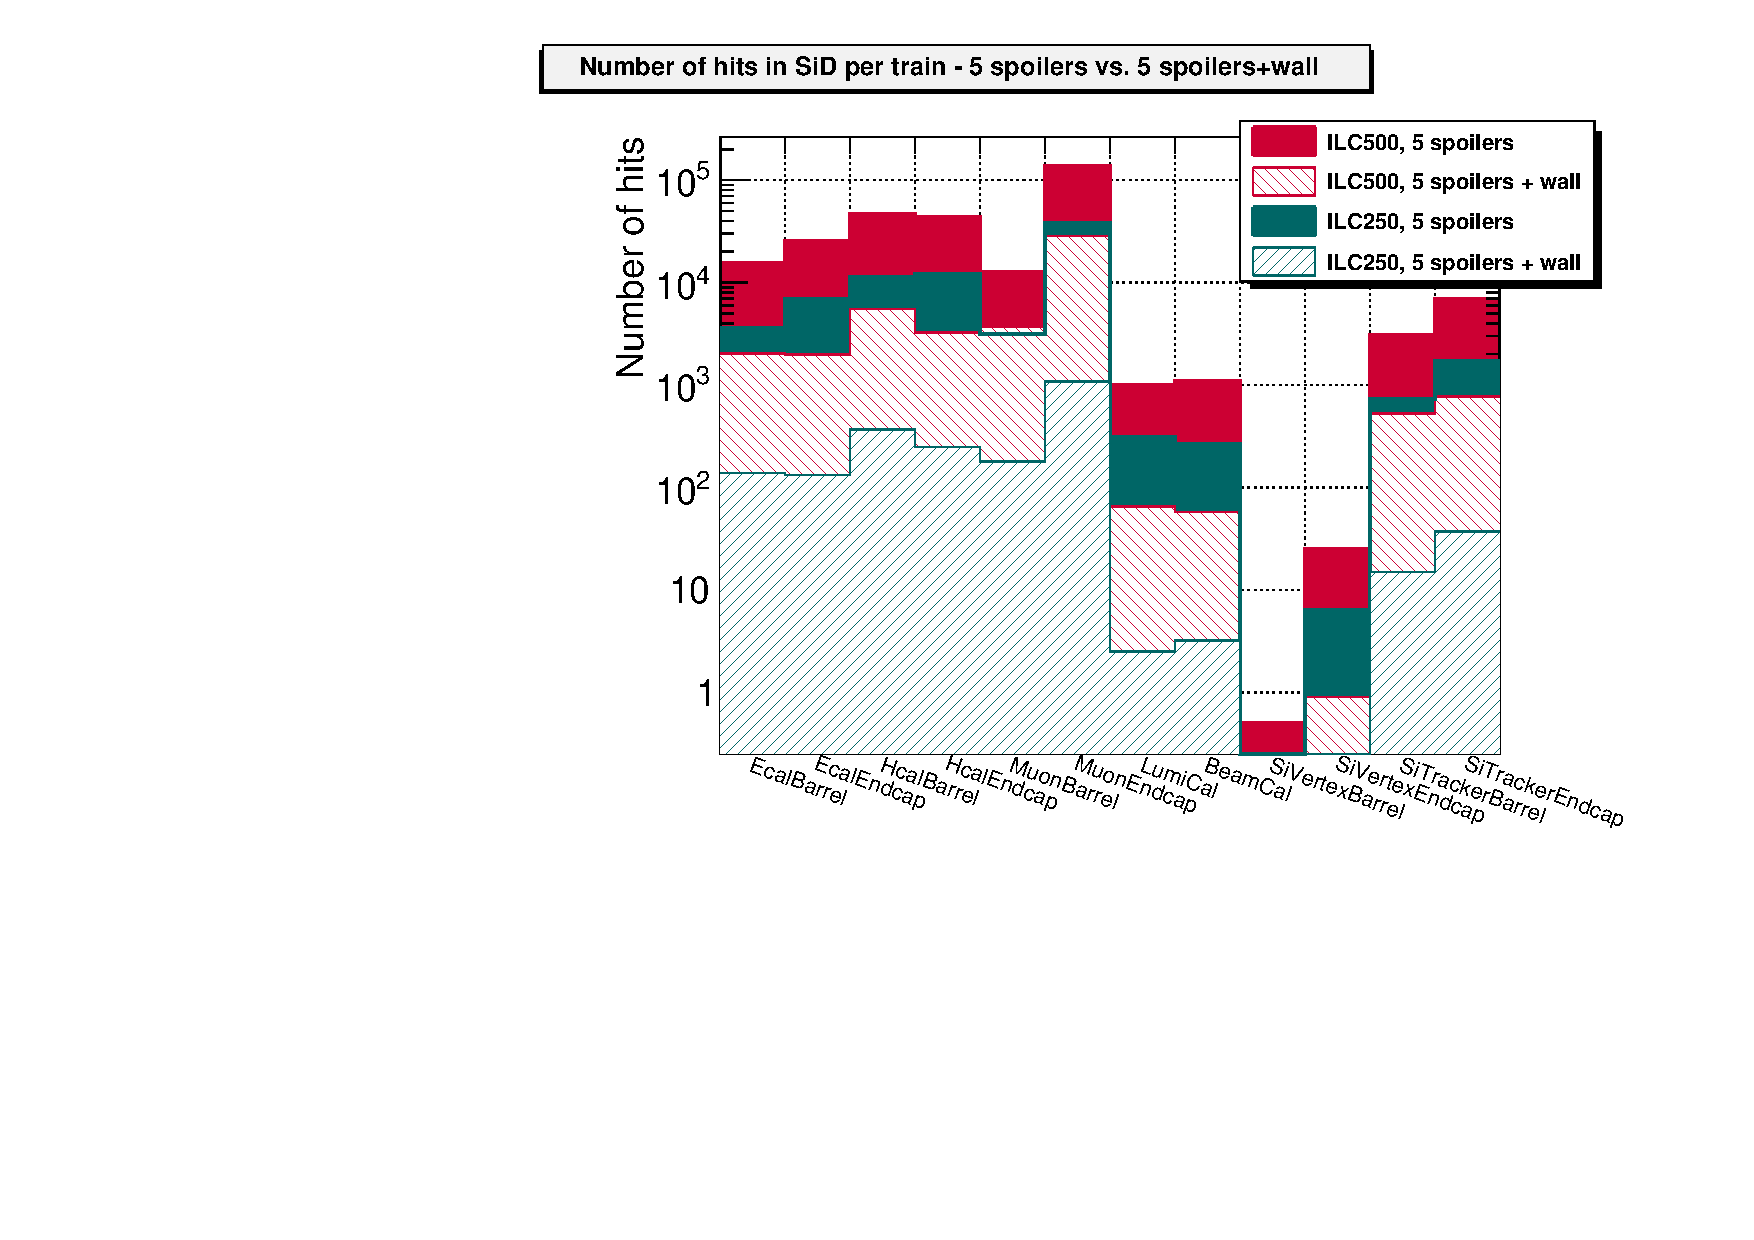
\includegraphics[width=\textwidth]{muons_figures/figures/Hits_in_SiD_subdetectors_MuonSpoilerStudy.pdf}
 \end{column}
\end{columns}
\begin{center}
\begin{tabular}{@{}p{0.343\textwidth}p{0.01\textwidth}p{0.18\textwidth}p{0.01\textwidth}p{0.343\textwidth}p{0.001\textwidth}@{}}
 \centering Vertex detectors & < & \centering ECAL, HCAL & < & \centering MuonEndcaps & \\
  \centering{\scriptsize Smallest effective detector area} & &  \centering{\scriptsize Particle showers} & &  \centering{\scriptsize Biggest effective detector area}&
\end{tabular}
\end{center}
\end{frame}


\subsubsection{Analysis - Occupancies}

\begin{frame}{Occupancy plots - \small HcalBarrel}
\sidlogo
{\footnotesize The following occupancy plots are normalized by the total number of cells.}\\\vspace*{0.1cm}
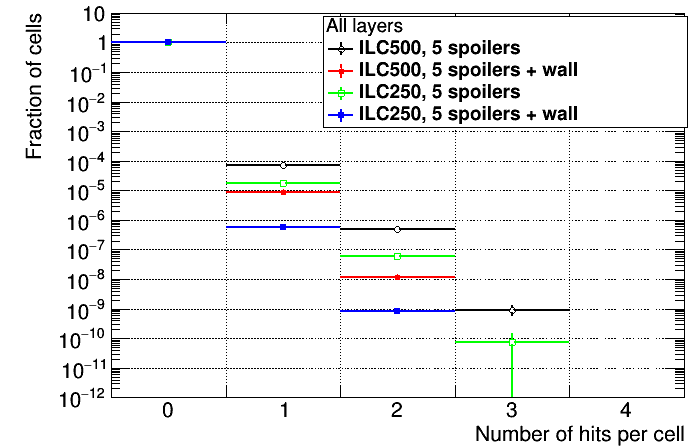
\includegraphics[height=0.46\textheight]{Occupancy_Comparison_All_layers_wrt_cells_HcalBarrel.pdf}\hfill
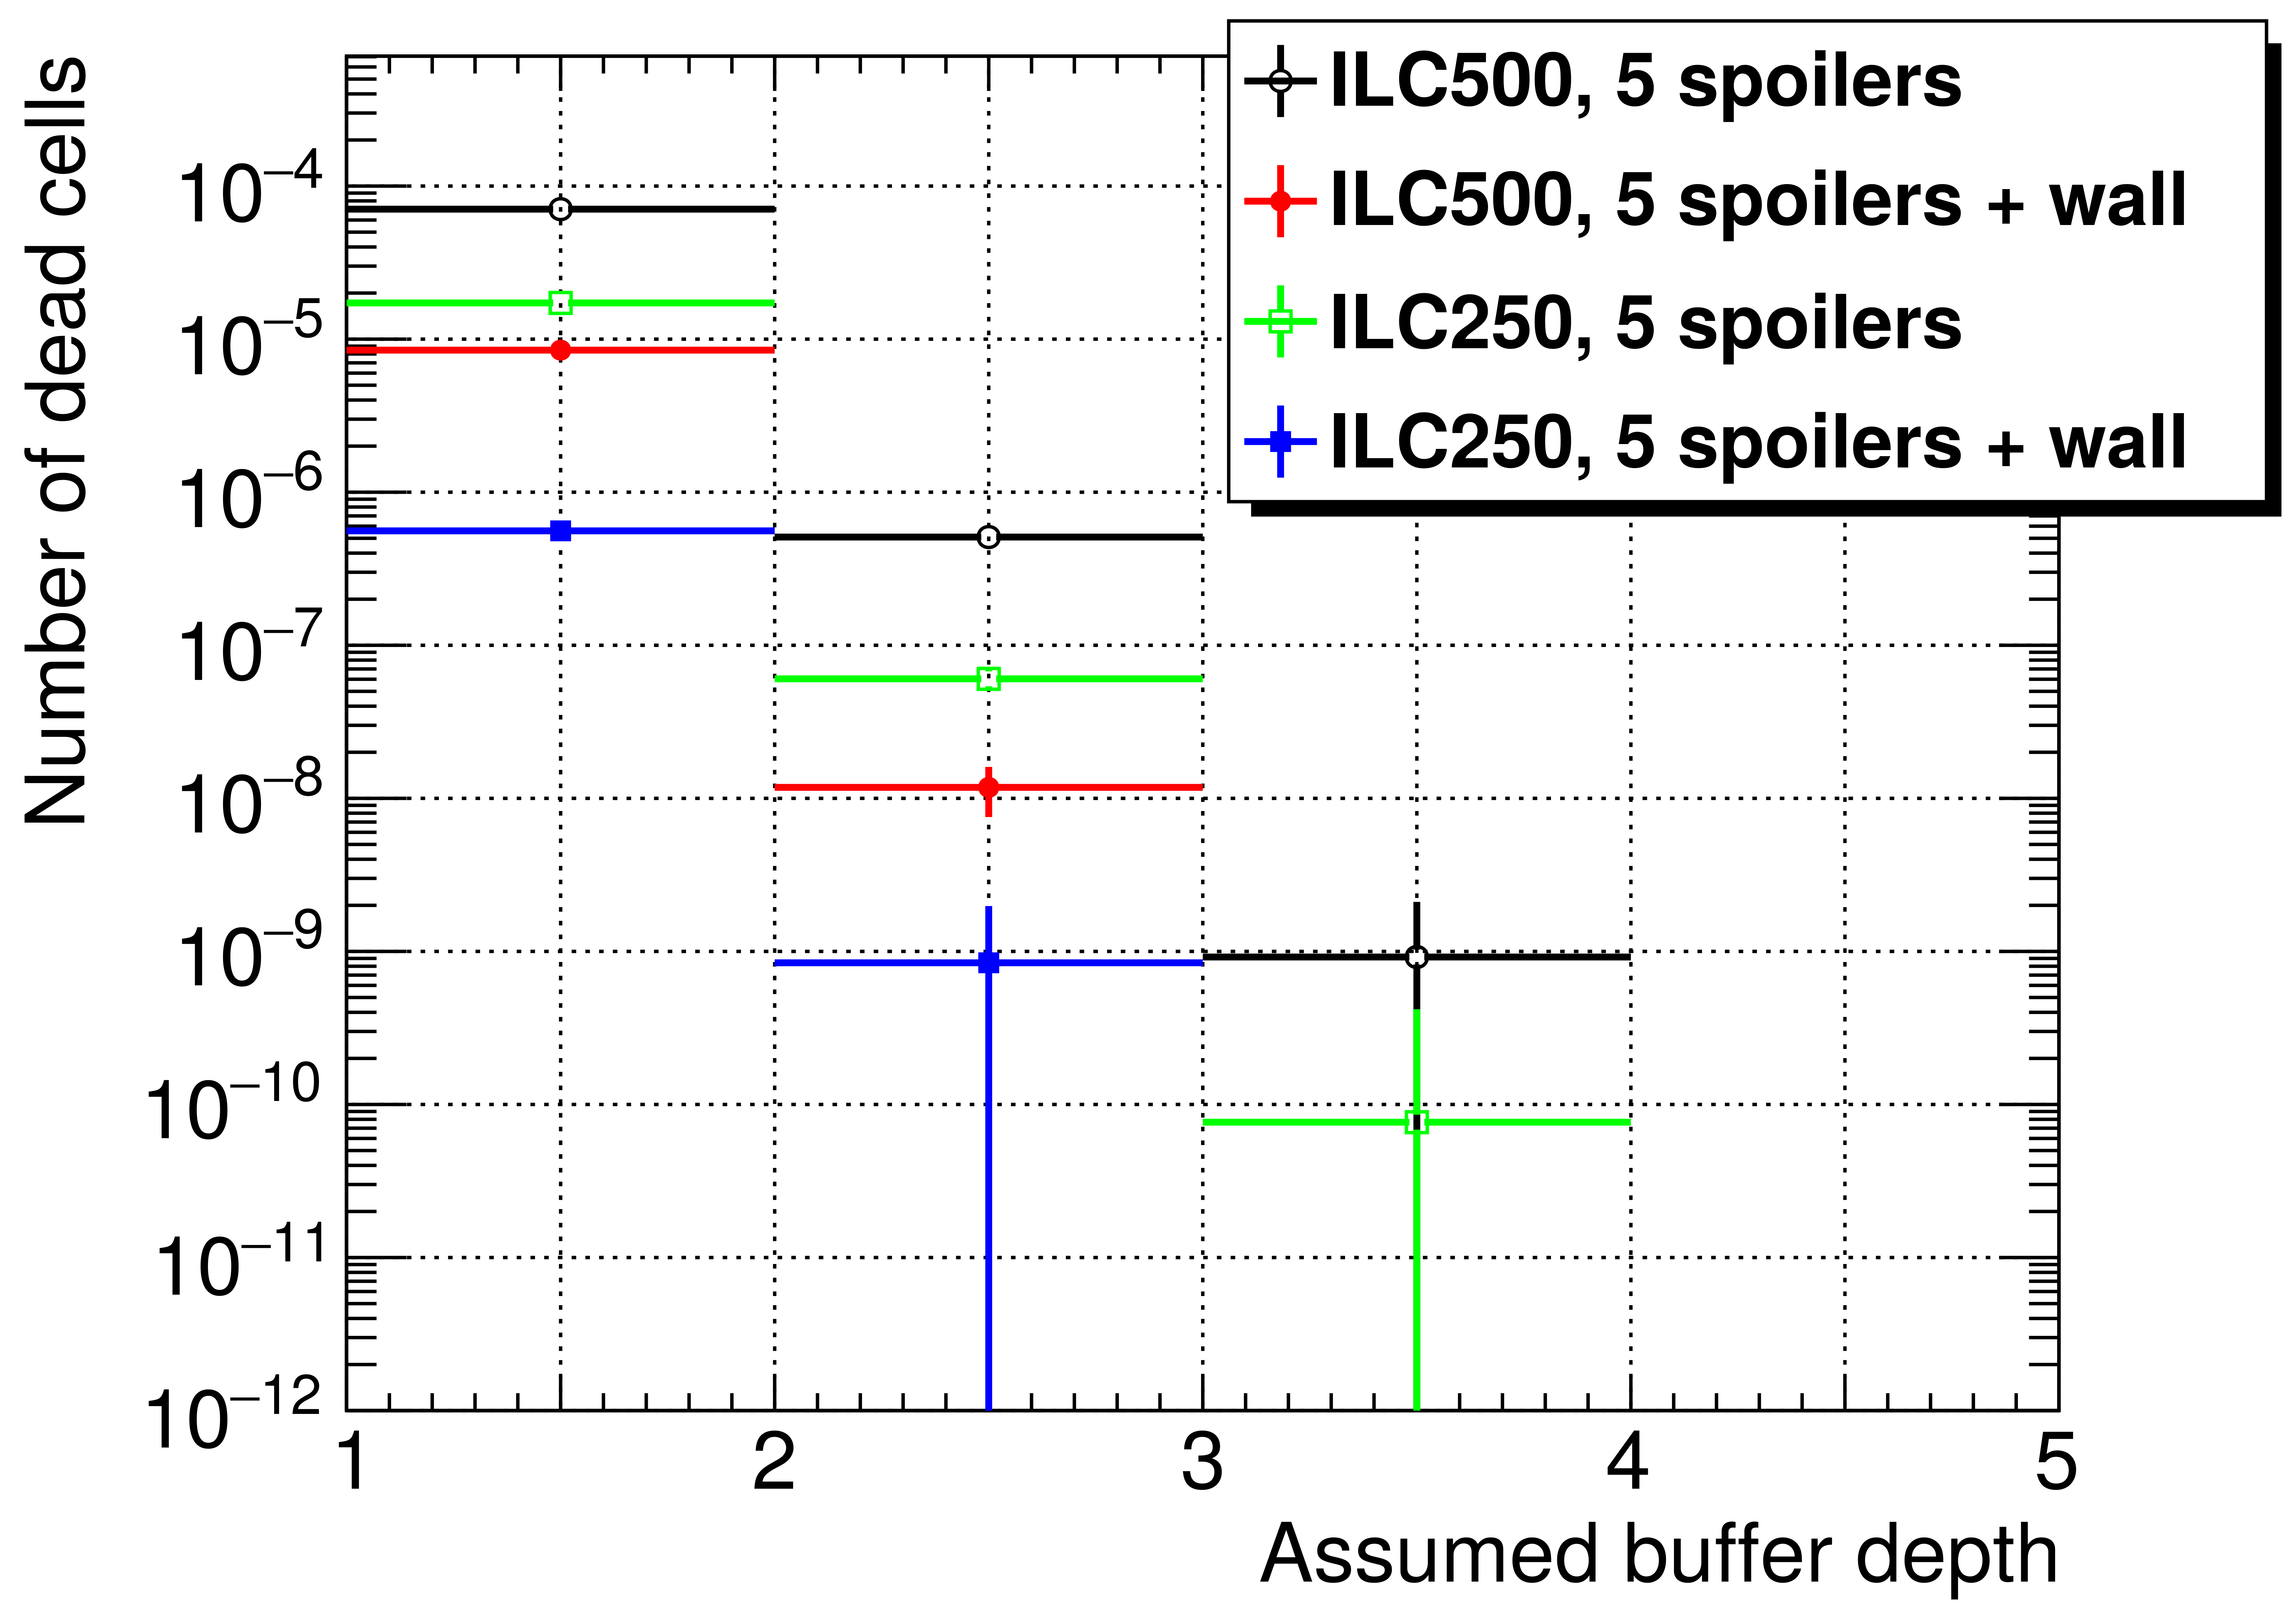
\includegraphics[height=0.46\textheight]{Occupancy_Comparison_All_layers_deadcells_HcalBarrel.pdf}\\
\vspace*{0.2cm}
Only up to three hits per cell $\rightarrow$ Low occupancy
\\'5 Spoilers + Wall' for 250 and 500\,GeV does better by up to an order of magnitude.
\end{frame}

\subsubsection{Analysis - Dead cells}
\begin{frame}{Occupancy plots - \small SiTrackerEndcap}
\sidlogo
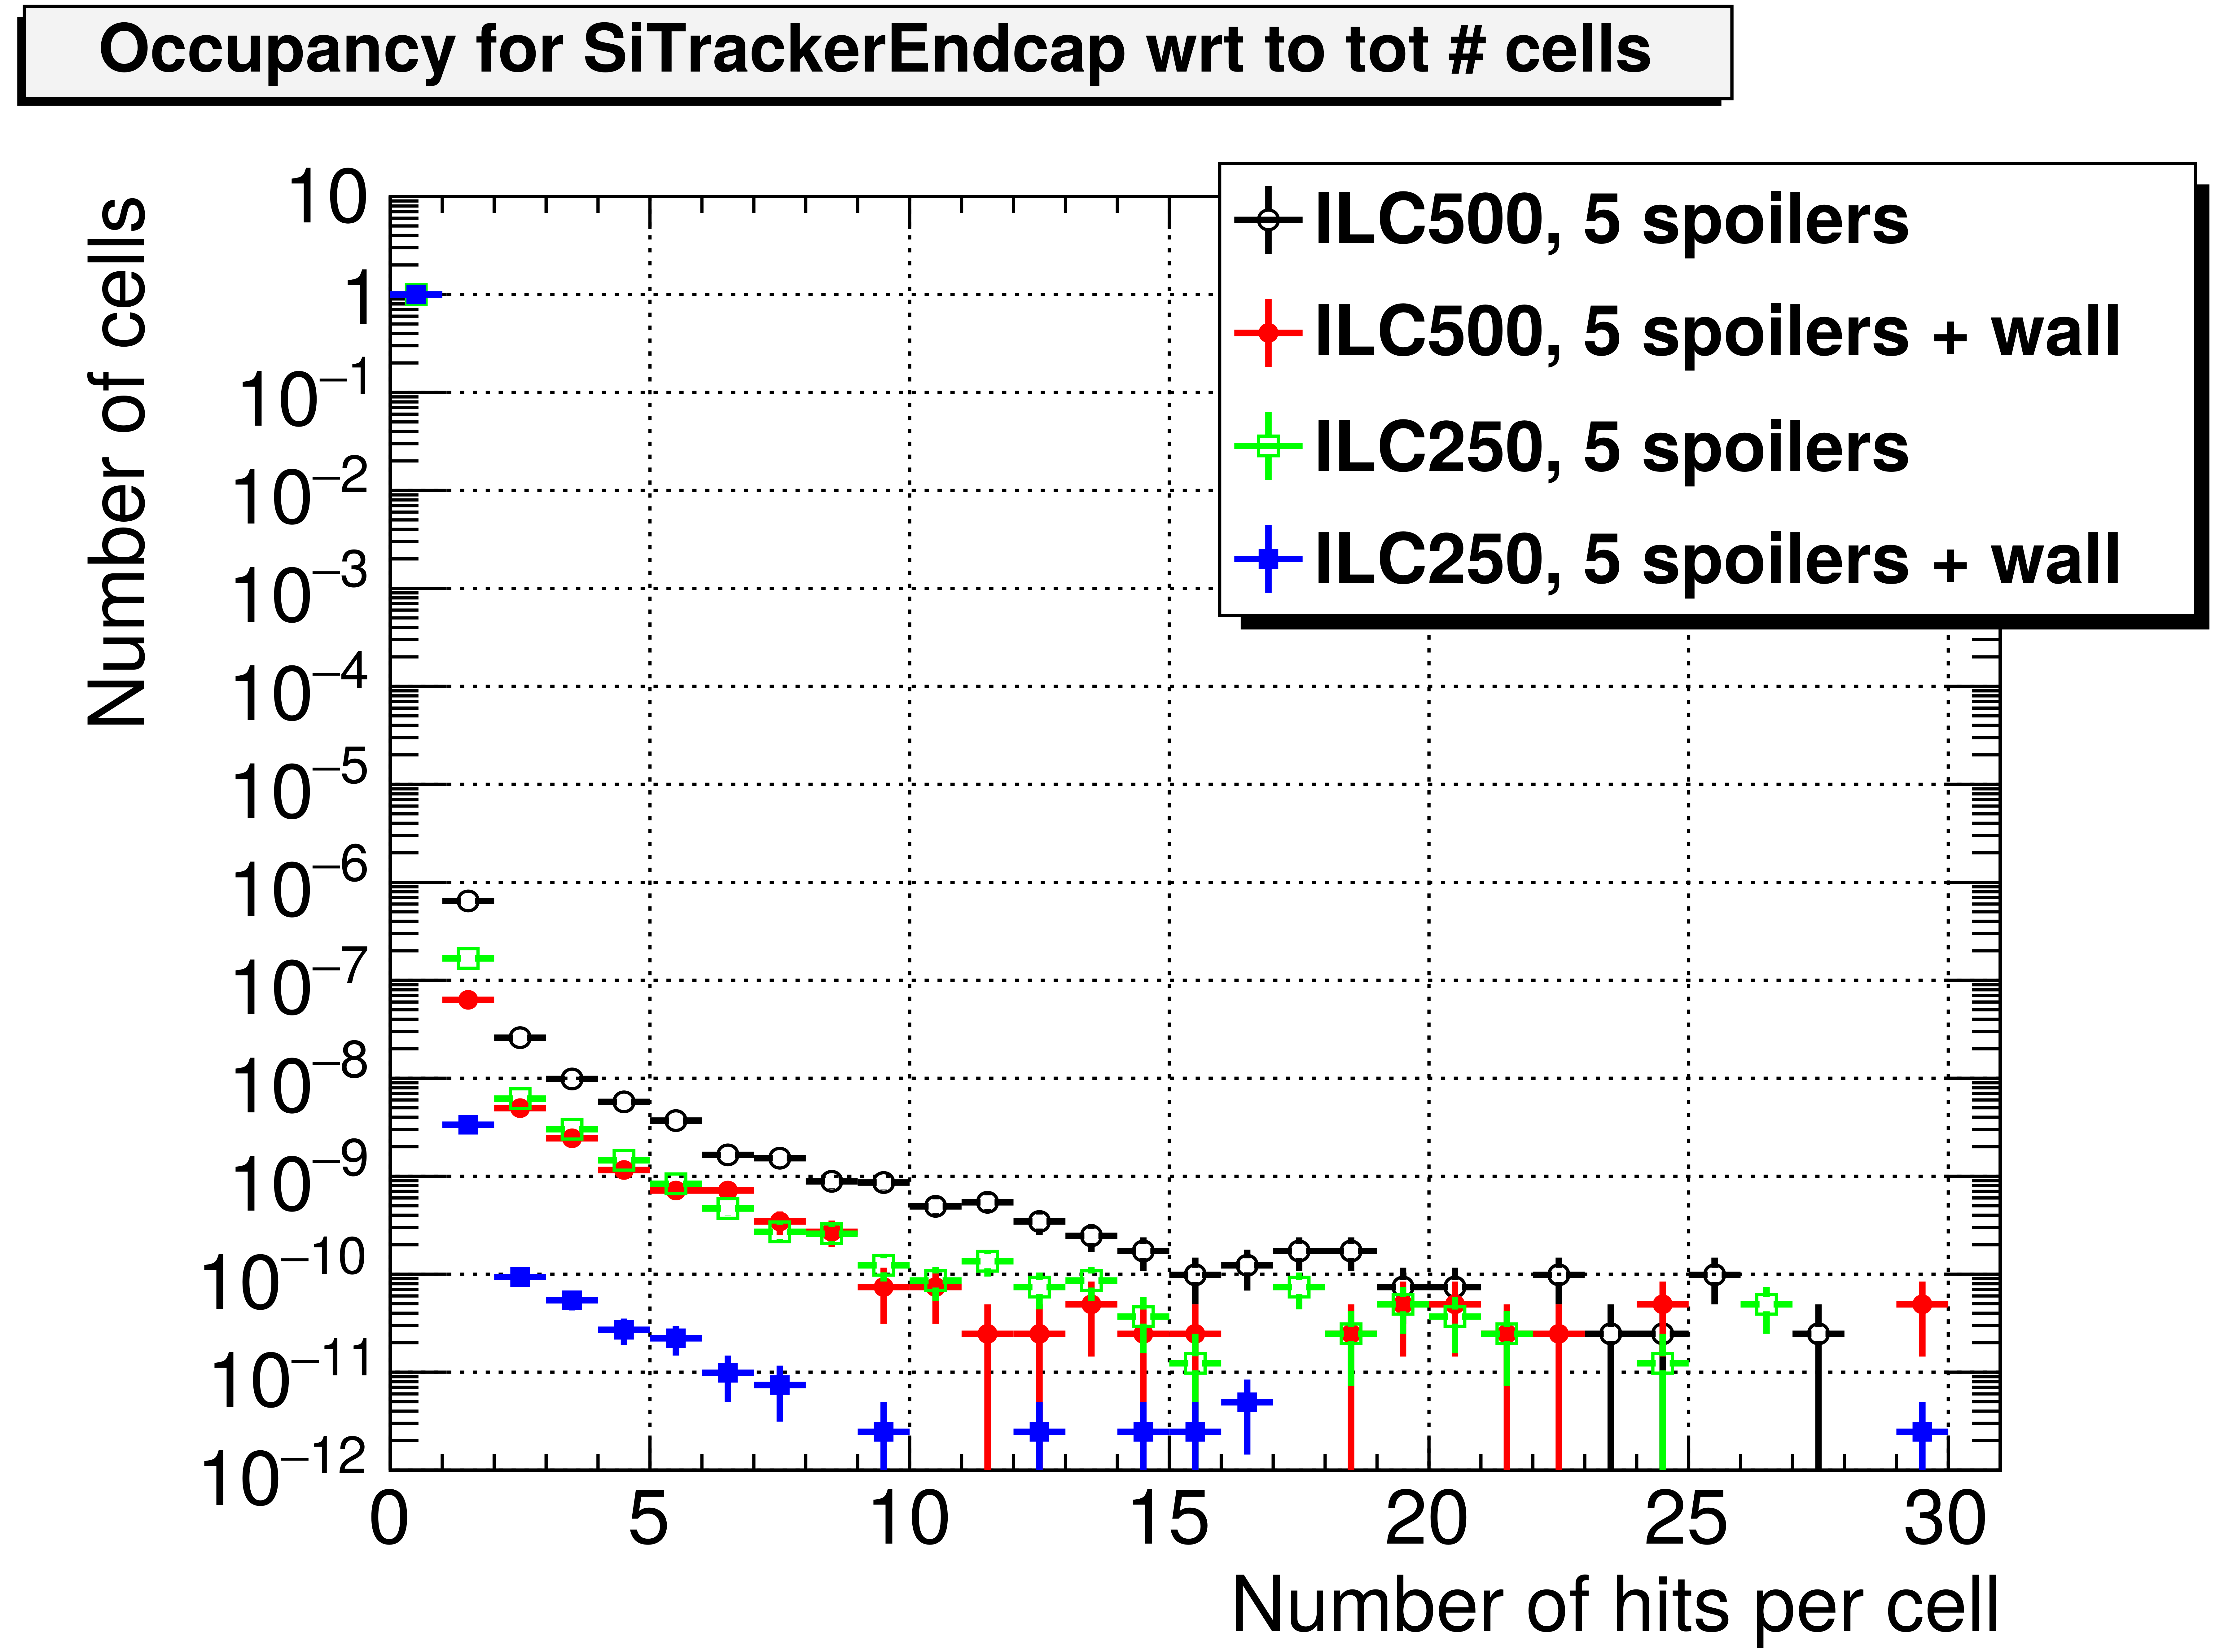
\includegraphics[height=0.46\textheight]{Occupancy_Comparison_All_layers_wrt_cells_SiTrackerEndcap.pdf}\hfill
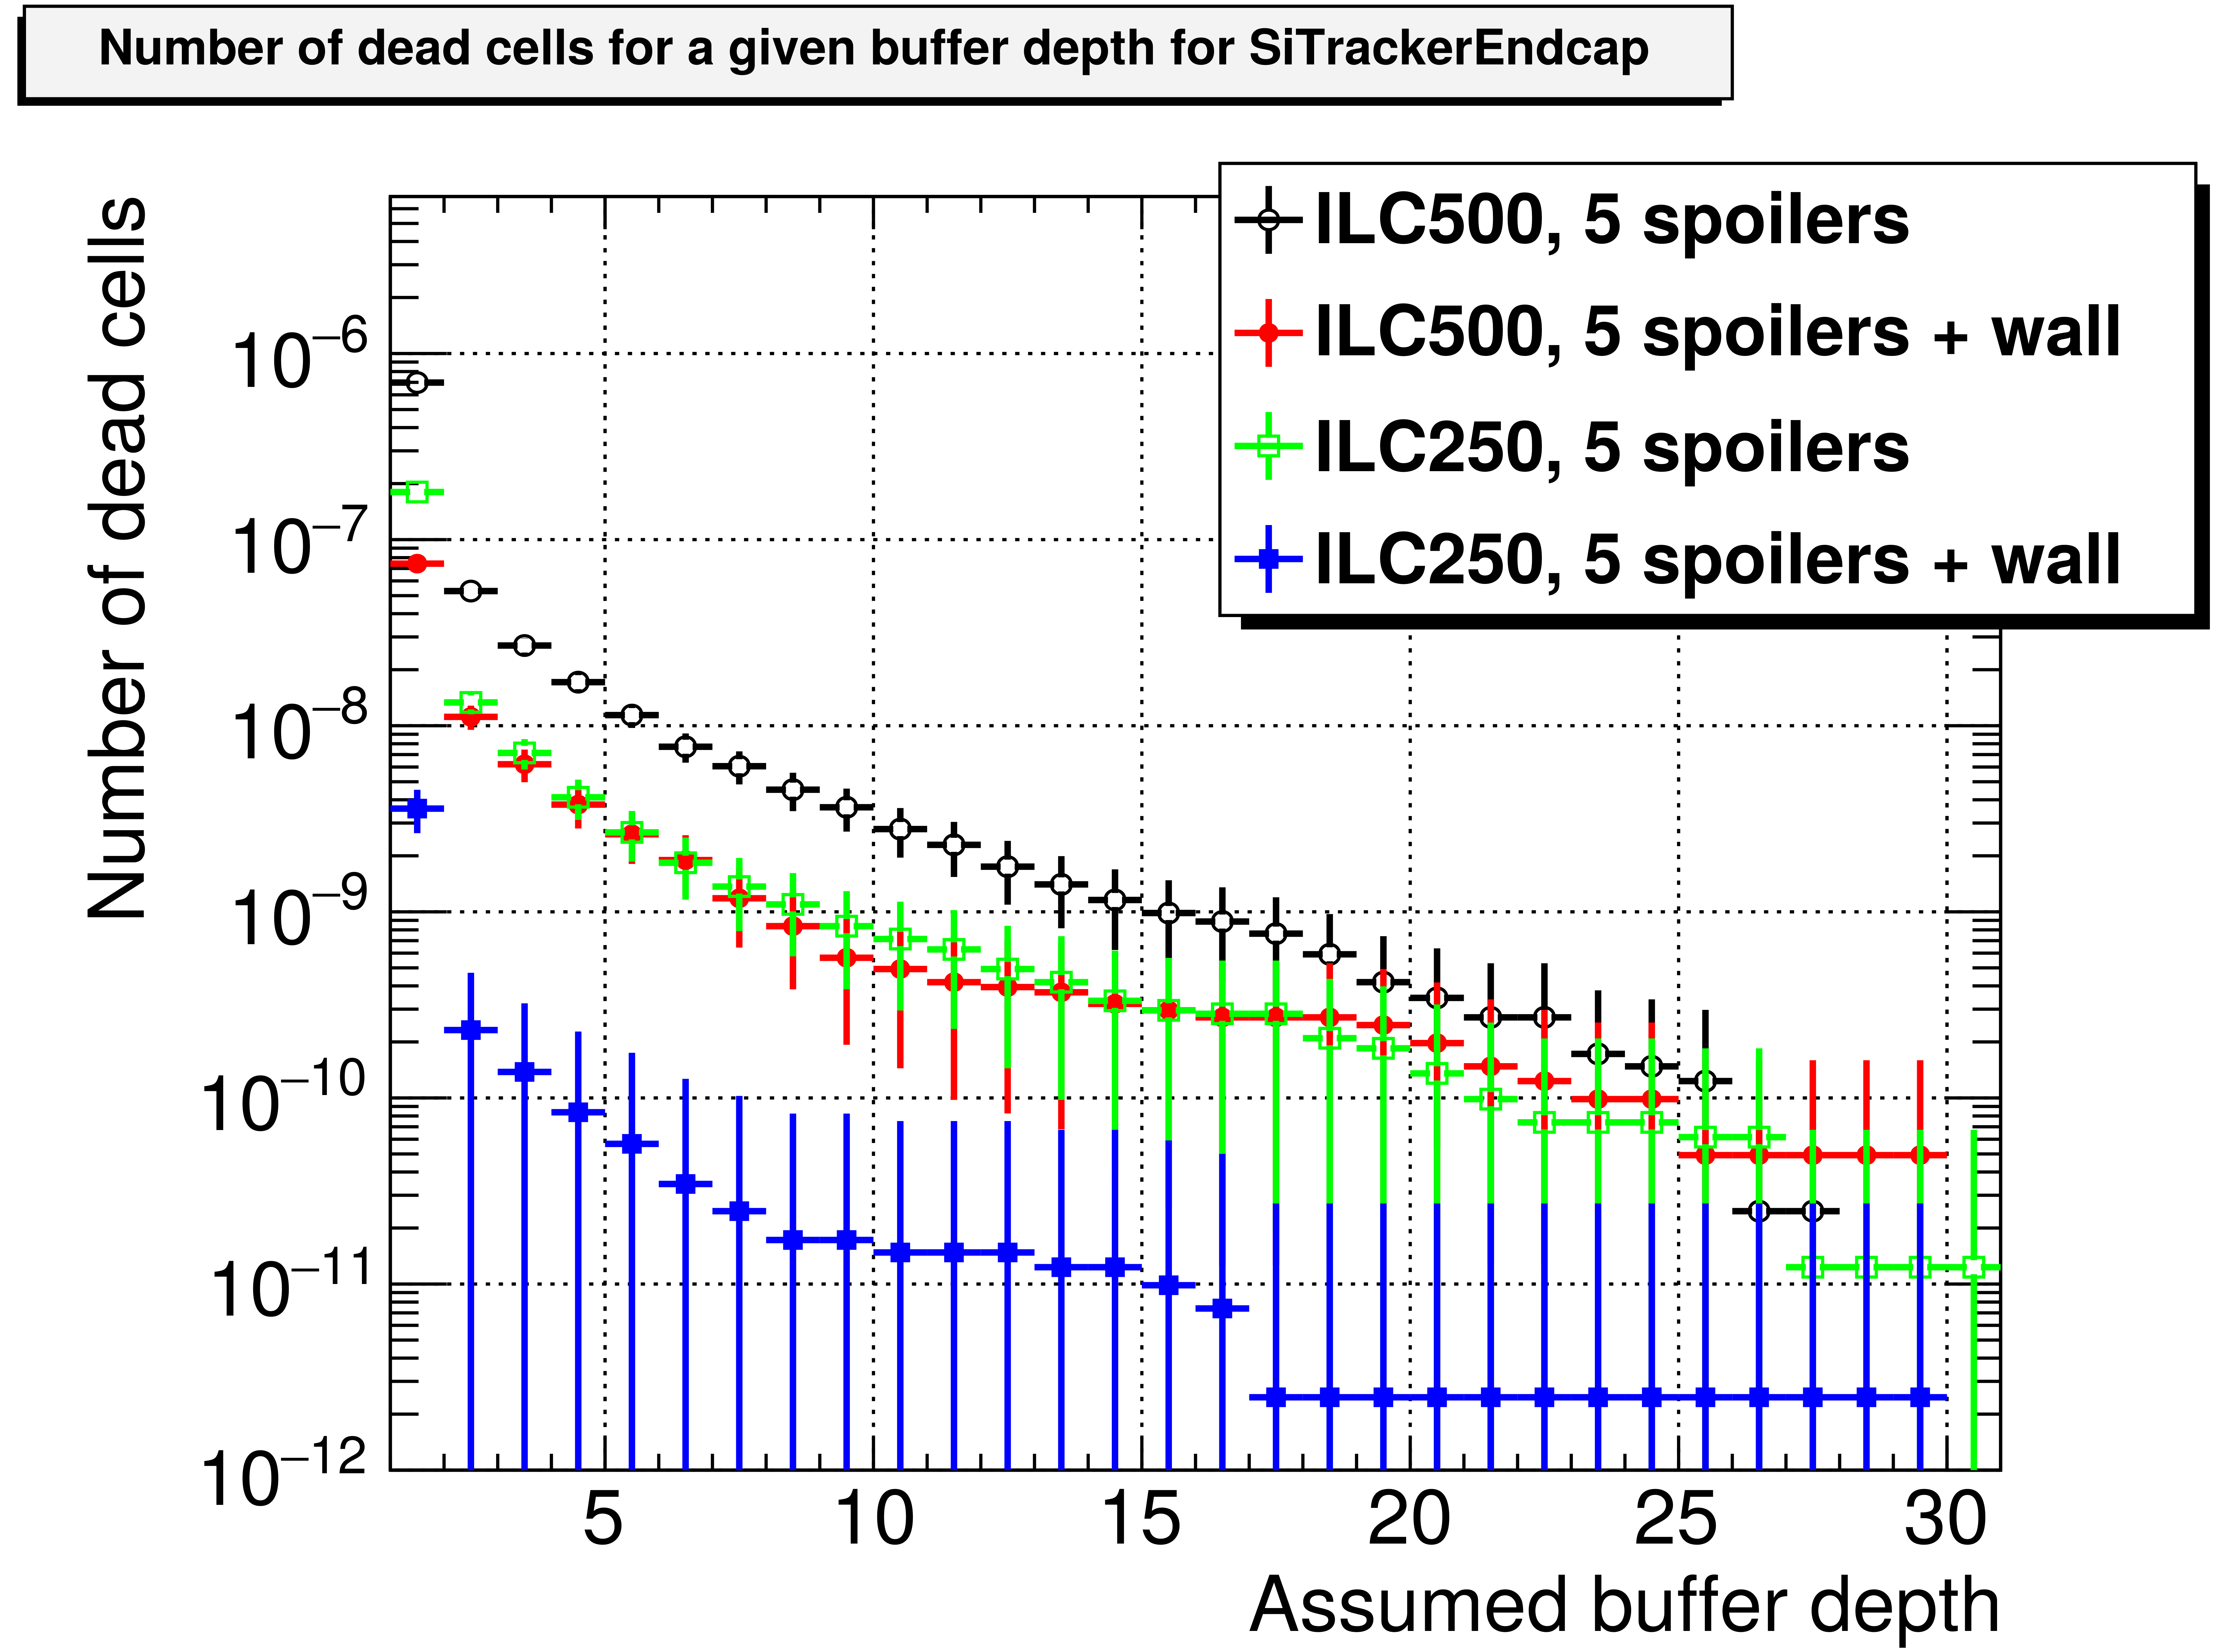
\includegraphics[height=0.46\textheight]{Occupancy_Comparison_All_layers_deadcells_SiTrackerEndcap.pdf}\\
Number of hits per cell up to 30 $\rightarrow$ low energy muons spiral, and hit cells several times!
\\For all assumed buffer depth values, the total number of dead cells stays way below 10$^{-4}$ (critical limit).
\end{frame}

\subsection{Conclusion}
\begin{frame}
\textit{Updated analysis framework and new numbers for ILC250 have shown:}
\begin{itemize}
 \item Muons penetrate the whole detector horizontally.
 \item At \alert{500\,GeV}, the \alert{5 spoilers} can reduce the number of muons to $\sim$4/bunch crossing, which results in \alert{occupancies of around $\sim10^{-4}$ (limit of acceptance)}.
 \item The 5 spoilers + wall scenario reduces this significantly.
 \item In the \alert{ILC250 stage}, the number of \alert{muons/bunch crossing is reduced by about a factor of 2}.
 \item The \alert{occupancies} are for both shielding scenarios \alert{well below $\sim10^{-4}$}.
\end{itemize}
\textit{Conclusion:}
\begin{itemize}
\item High energy muons could be used for tracker alignment.
\item Spatial distributions quite different in scenarios w/ \& w/o the wall.
\item \alert{With the shown evaluation of the muons from the current MUCARLO simulations, the \alert{magnetized wall is not required for limiting the detector occupancy in the ILC250 stage}.
However, the wall serves as a tertiary containment device, and might be mandatory anyway.}
\end{itemize}
\end{frame}


%--------------------------------------------------------------------------------------------------------------

\section{FLUKA simulation of the ILC Beam Dump}

{
\usebackgroundtemplate{
\vbox to \paperheight{\vfil
 \tikz\node[opacity=0.1]{\includegraphics[width=\paperwidth]{BeamDump_figures/TB-0067-300-00-A_yz_view.png}};
 \vfil}
}
\begin{frame}{Neutron Background and Beam Dump Irradiation}
\flukalogo
The 17\,MW\footnote{13.7\,MW average beam power + 20\% margin} beam is dumped into a water tank after collision.\\The activation of the dump surrounding will permit access to the dump area. Neutrons ($\lesssim$\SI{e10}{\per\square\centi\metre\per\year}) are emitted that irradiate the surroundings, and travel back towards the detectors.~\cite{SLAC_FLUKA}\\
\vspace*{0.5cm}
\alert{Goal: Simulating the energy deposition, irradiation, and background particles:}
\\$\rightarrow$Simulating the activation, and the neutrons from the beam dump with FLUKA, using the design drawings by B. Smith~\cite{Smith} to model the dump and the surrounding.

\end{frame}
}

\subsection{The Beam Dump Designs}
{\usebackgroundtemplate{
\vbox to \paperheight{\vspace*{1.2cm}
 \tikz\node[opacity=0.3]{\hspace*{0.6cm} \includegraphics[width=0.92\textwidth]{BeamDump_figures/TB-0067-210-00-A.png}};
 \vfil}}
\begin{frame}{\textbf{Design 1}: 0-TB-0067-210-00-A}
Design drawings by B. Smith, 2006-2007~\cite{Smith}\vspace*{0.3cm}
\begin{columns}
 \begin{column}{0.5\textwidth}
  Vessel:
  \begin{itemize}
   \item Diameter: 1.5\,m
   \item Length: 6.5\,m
   \item 316L Stainless Steel
   \item Water pressure: 10\,bar
  \end{itemize}
  Window:
  \begin{itemize}
   \item Diameter: 300\,mm
   \item Thickness: 1\,mm
   \item Titanium alloy: Ti-6Al-4V 
  \end{itemize}
 \end{column}
 \begin{column}{0.5\textwidth}
  27\,X\textsubscript{0} needed to stop a 500\,GeV beam:
  \begin{itemize}
   \item Water: 18\,X\textsubscript{0}
   \item Water cooled copper plates: 9\,X\textsubscript{0} = 126\,mm
  \end{itemize}  
 \end{column}
\end{columns}

\end{frame}
}

{
\usebackgroundtemplate{
\vbox to \paperheight{\vspace*{1.2cm}
 \tikz\node[opacity=0.3]{\hspace*{0.6cm} \includegraphics[width=0.92\textwidth]{BeamDump_figures/TB-0067-300-00-A.png}};
 \vfil}}
\begin{frame}{\textbf{Design 2}: 0-TB-0067-210-00-A}
Design drawings by B. Smith, 2006-2007~\cite{Smith}\vspace*{0.3cm}
\begin{columns}
 \begin{column}{0.5\textwidth}
  Vessel:
  \begin{itemize}
   \item Diameter: 1.5\,m
   \item Length: 6.5\,m
   \item 316L Stainless Steel
   \item Water pressure: 10\,bar
  \end{itemize}
  Window:
  \begin{itemize}
   \item Diameter: 300\,mm
   \item Thickness: 1\,mm
   \item Titanium alloy: Ti-6Al-4V 
  \end{itemize}
 \end{column}
 \begin{column}{0.5\textwidth}
  27\,X\textsubscript{0} needed to stop a 500\,GeV beam:
  \begin{itemize}
   \item Water: 18\,X\textsubscript{0}
   \item Water cooled copper plates: 9\,X\textsubscript{0} = 126\,mm
  \end{itemize}  
    \alert{Additionally high water pressure section:}
  \begin{itemize}
   \item Titanium tubes, 4\,cm diameter
   \item High pressure water flow
   \item In total 1.98\,X\textsubscript{0}
  \end{itemize} 
 \end{column}
\end{columns}

\end{frame}
}

\subsection{The FLUKA simulation}
\begin{frame}
For the simulation, the ILC1000B was chosen as the scenario with the largest beam power.\\
\vspace*{0.5cm}
 ILC1000B:
 \begin{itemize}
  \item Beam energy: 500\,GeV
  \item Bunch population: $1.74\times10^{10}$
  \item Bunch size: \textsigma\textsubscript{x} = 2.4\,mm, \textsigma\textsubscript{y} = 0.22\,mm
  \item Bunches per train: 2450
  \item Bunch train duration: 896.7\,\textmu s
 \end{itemize}
\vspace*{0.2cm}
Beams are considered un-collided and un-disrupted.
\end{frame}


\subsubsection{Deposited Energy and Dose}
\begin{frame}{Deposited Energy per bunch}
\begin{center}
\hspace*{1.6cm} Design 1 \hfill Design 2 \hspace*{1.8cm} \\
  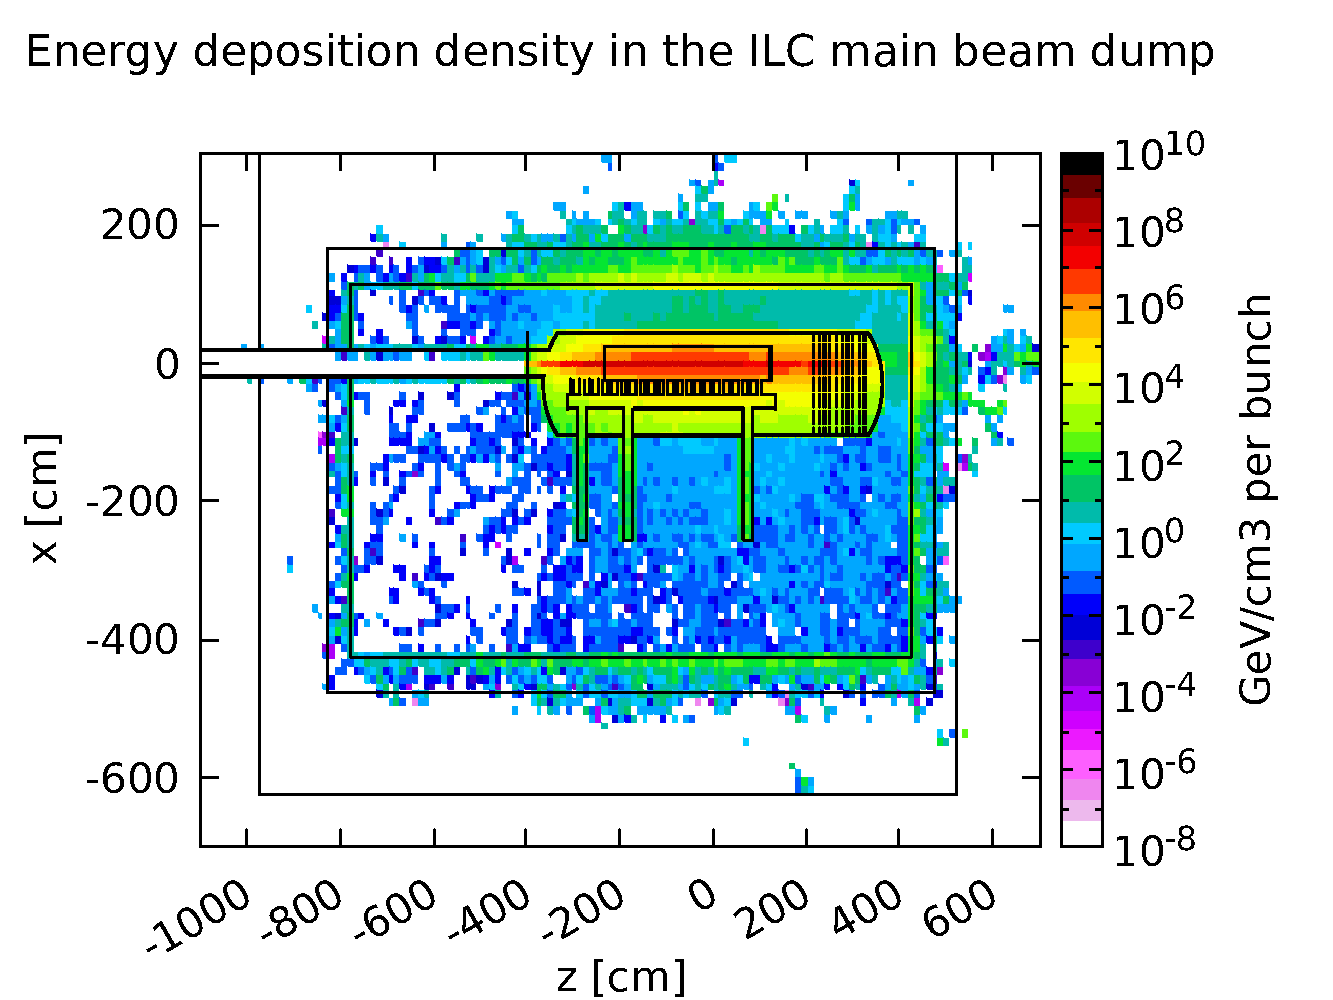
\includegraphics[width=0.52\textwidth]{BeamDump_figures/Energy_deposition_xz_Design1.pdf}
    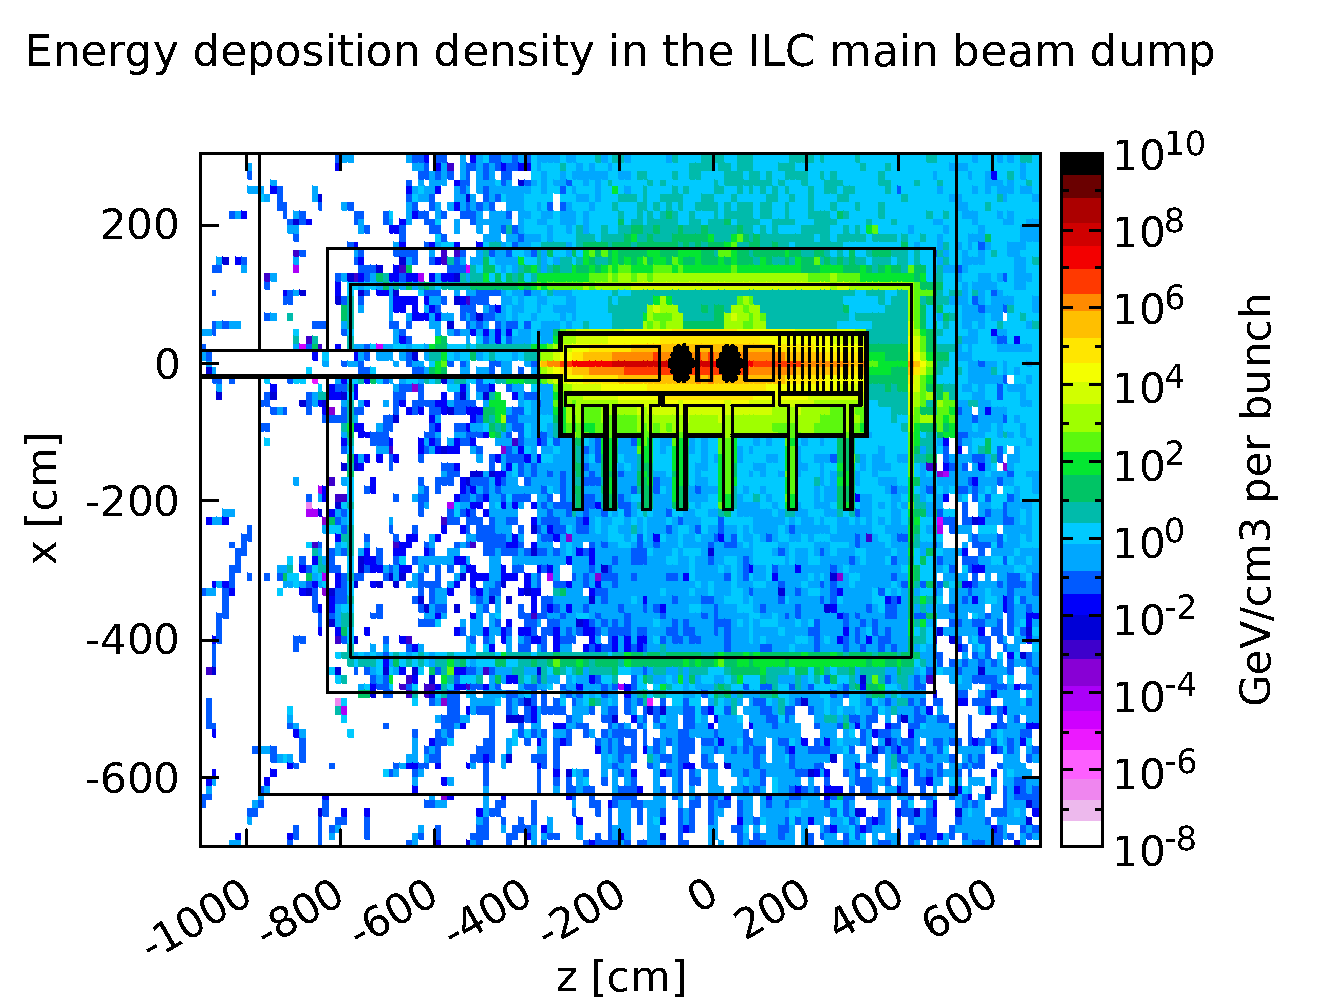
\includegraphics[width=0.52\textwidth]{BeamDump_figures/Energy_deposition_xz_Design2.pdf}
\end{center}
 Shielding walls seem to stop particles fluxes well, but large scattering in Design 2 at high water pressure sections leads to energy deposition outside the walls.
\end{frame}

\begin{frame}{Dose equivalent after cooling times}
\textbf{After one month of beam operation}, the beam is turned off.\\
  \begin{center}
    \hspace*{3cm} Instantaneous \hfill After 1 year \hspace*{2cm} \\
    \textbf{Design 1}
  \includegraphics[width=0.35\textwidth]{BeamDump_figures/Dose_equivalent_total_Design1.png}
  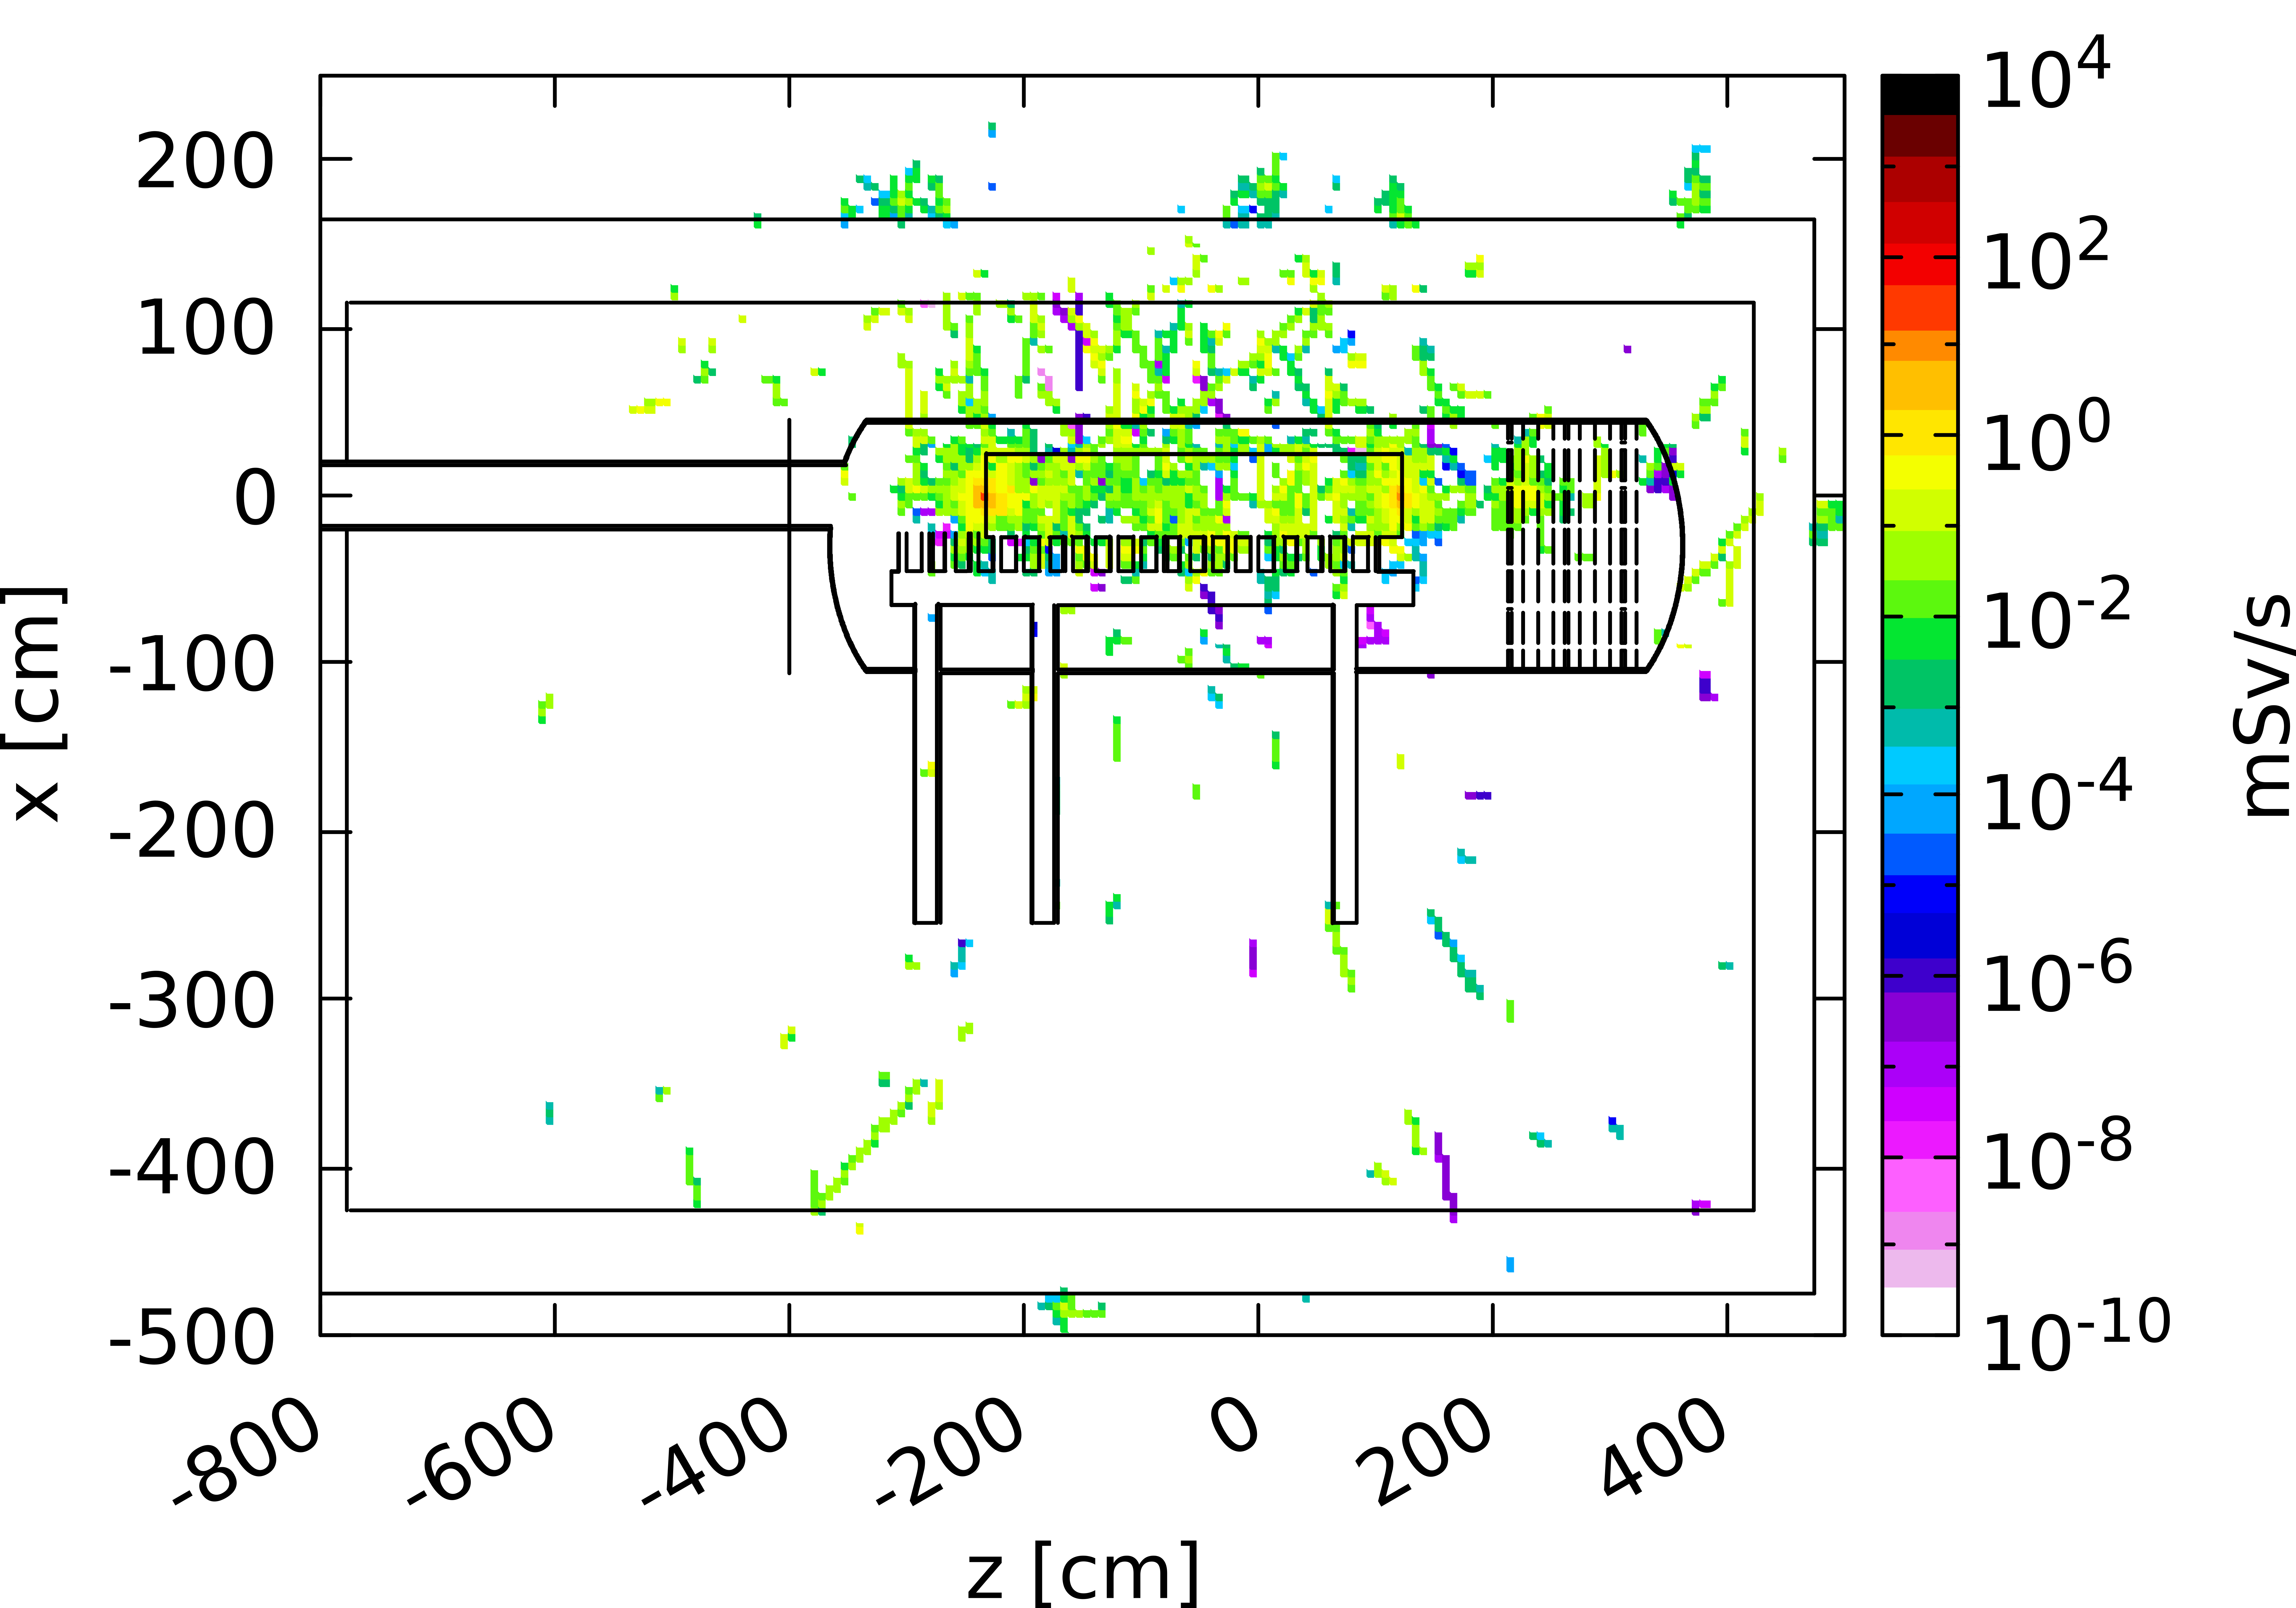
\includegraphics[width=0.35\textwidth]{DoseEQ_Time/Design1_5.png}
 \end{center}

  \begin{center}
    \textbf{Design 2}
  \includegraphics[width=0.35\textwidth]{BeamDump_figures/Dose_equivalent_total_Design2.png}
  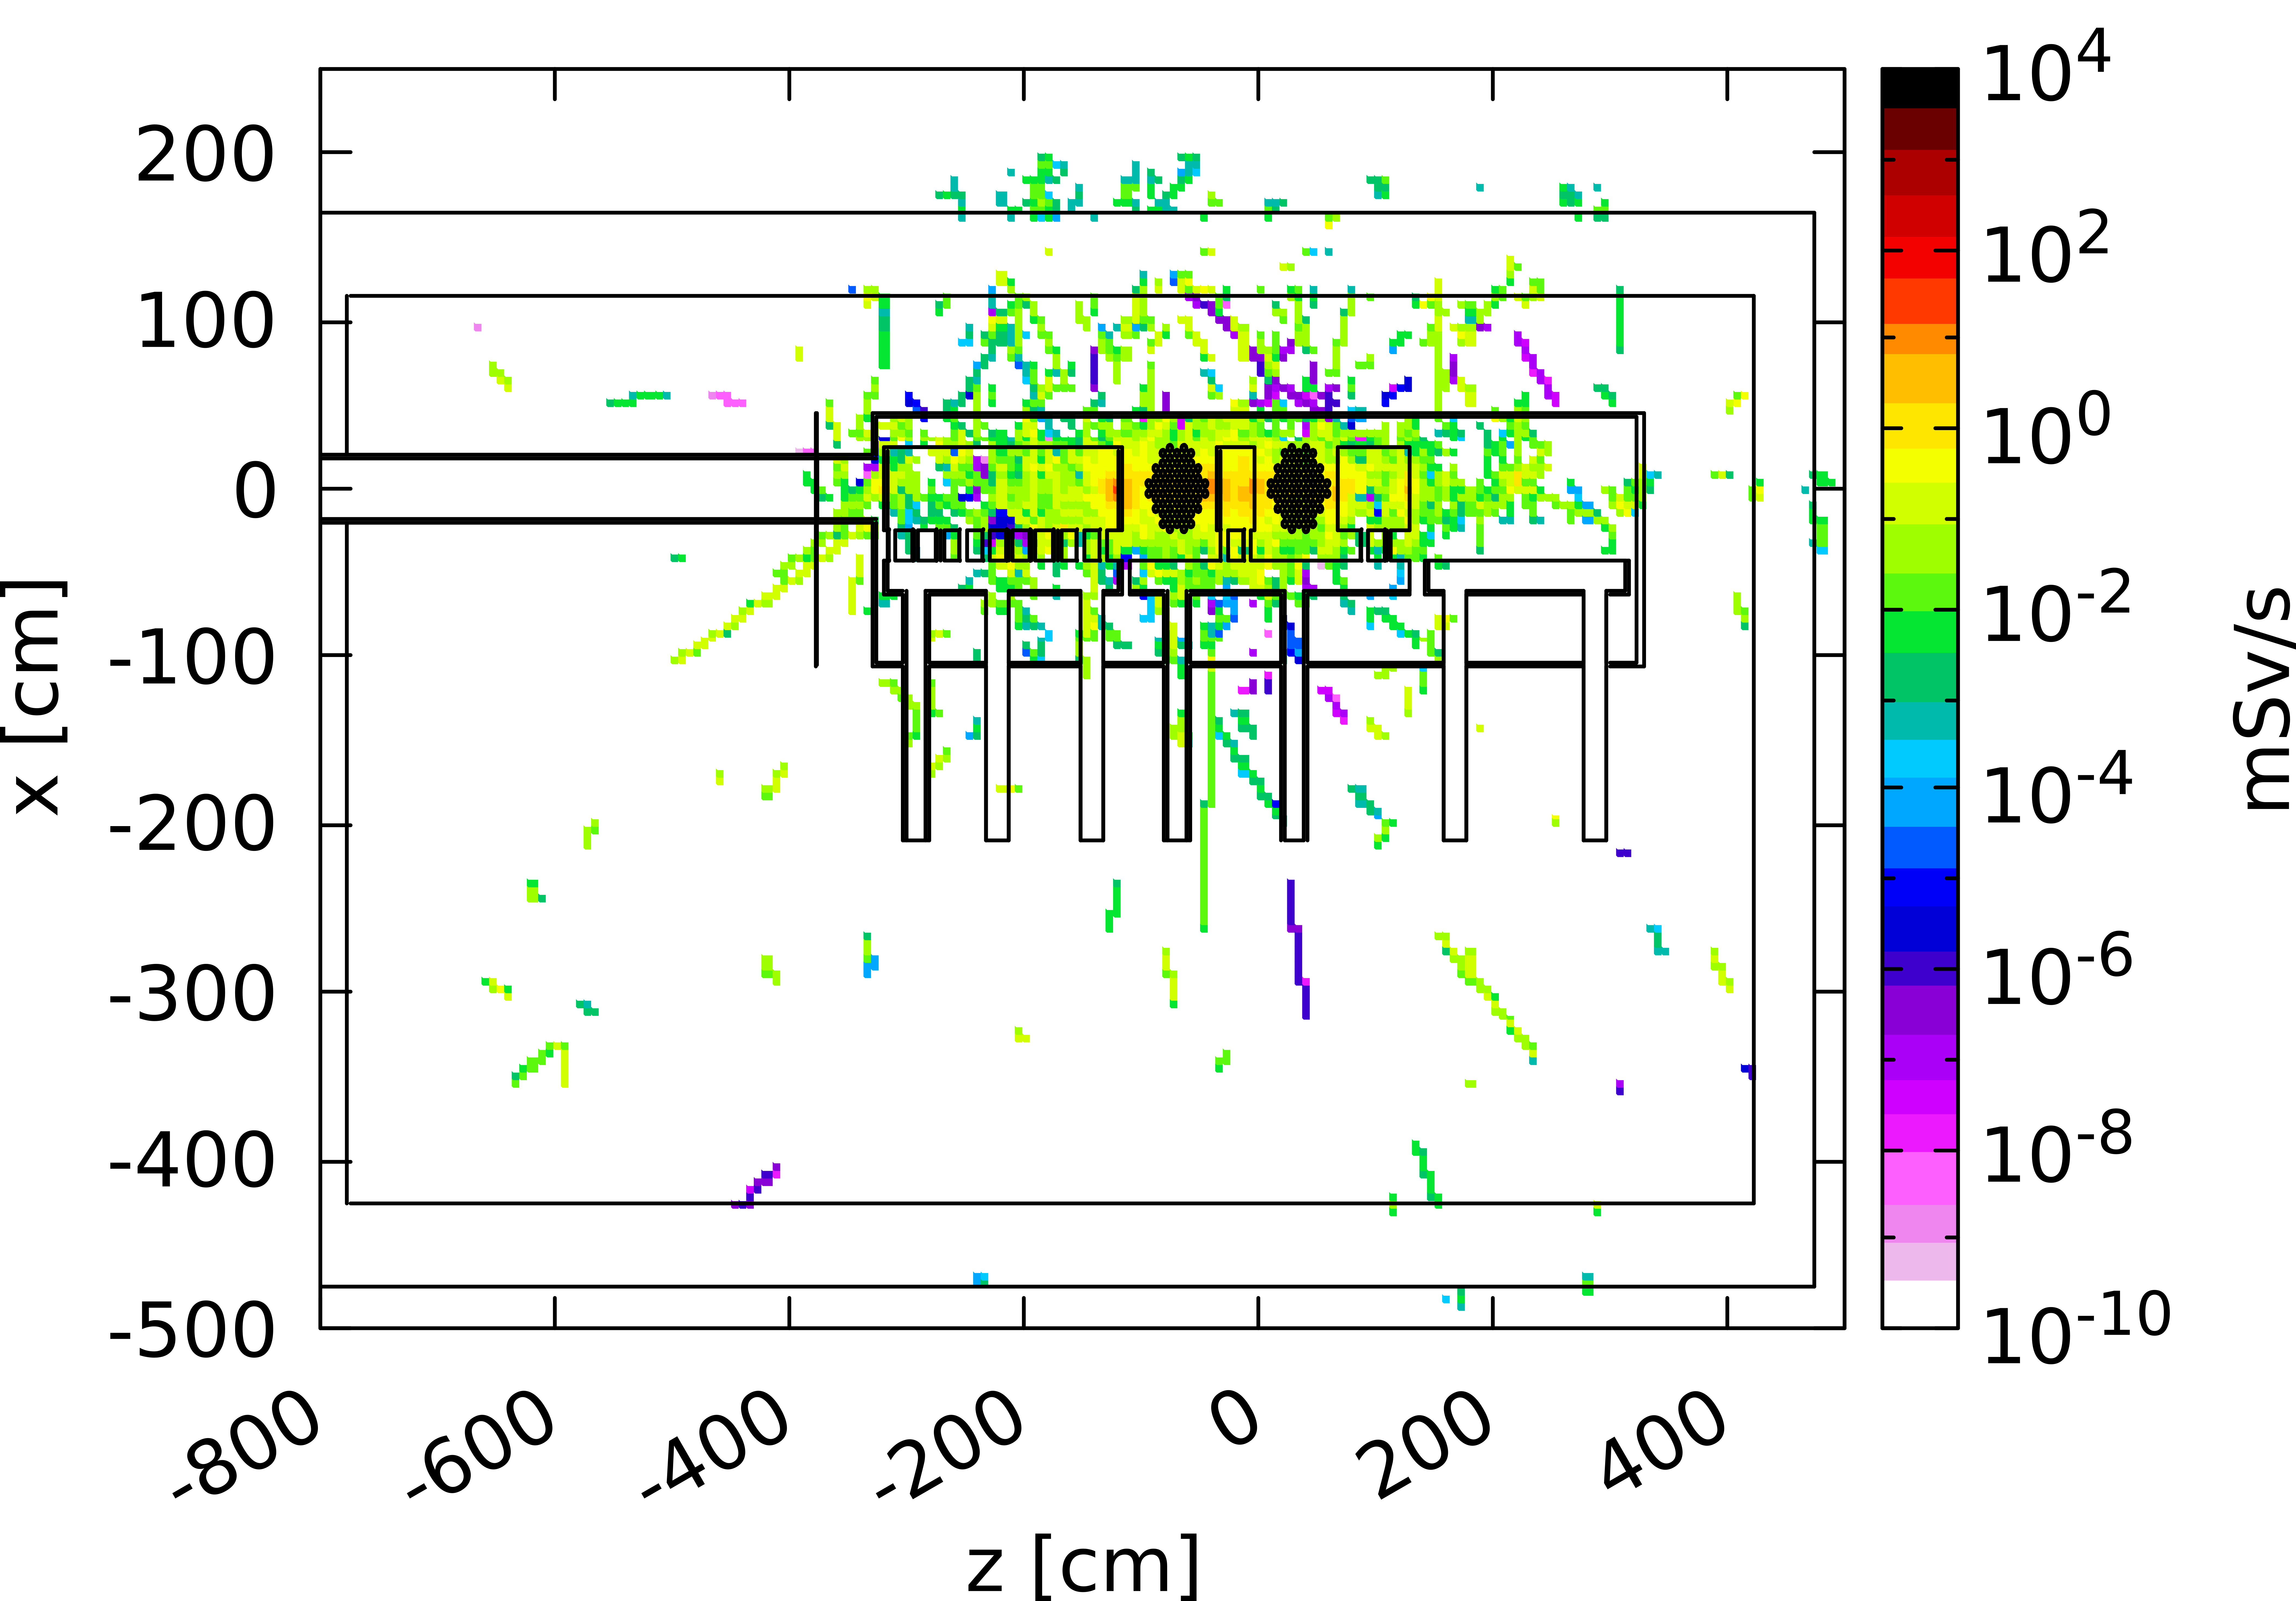
\includegraphics[width=0.35\textwidth]{DoseEQ_Time/Design2_5.png}
 \end{center}
\end{frame}
\begin{frame}{Dose Rate over Time}
The dose rate measured at the longitudinal shower maximum inside the vessel over time:
\begin{center}
  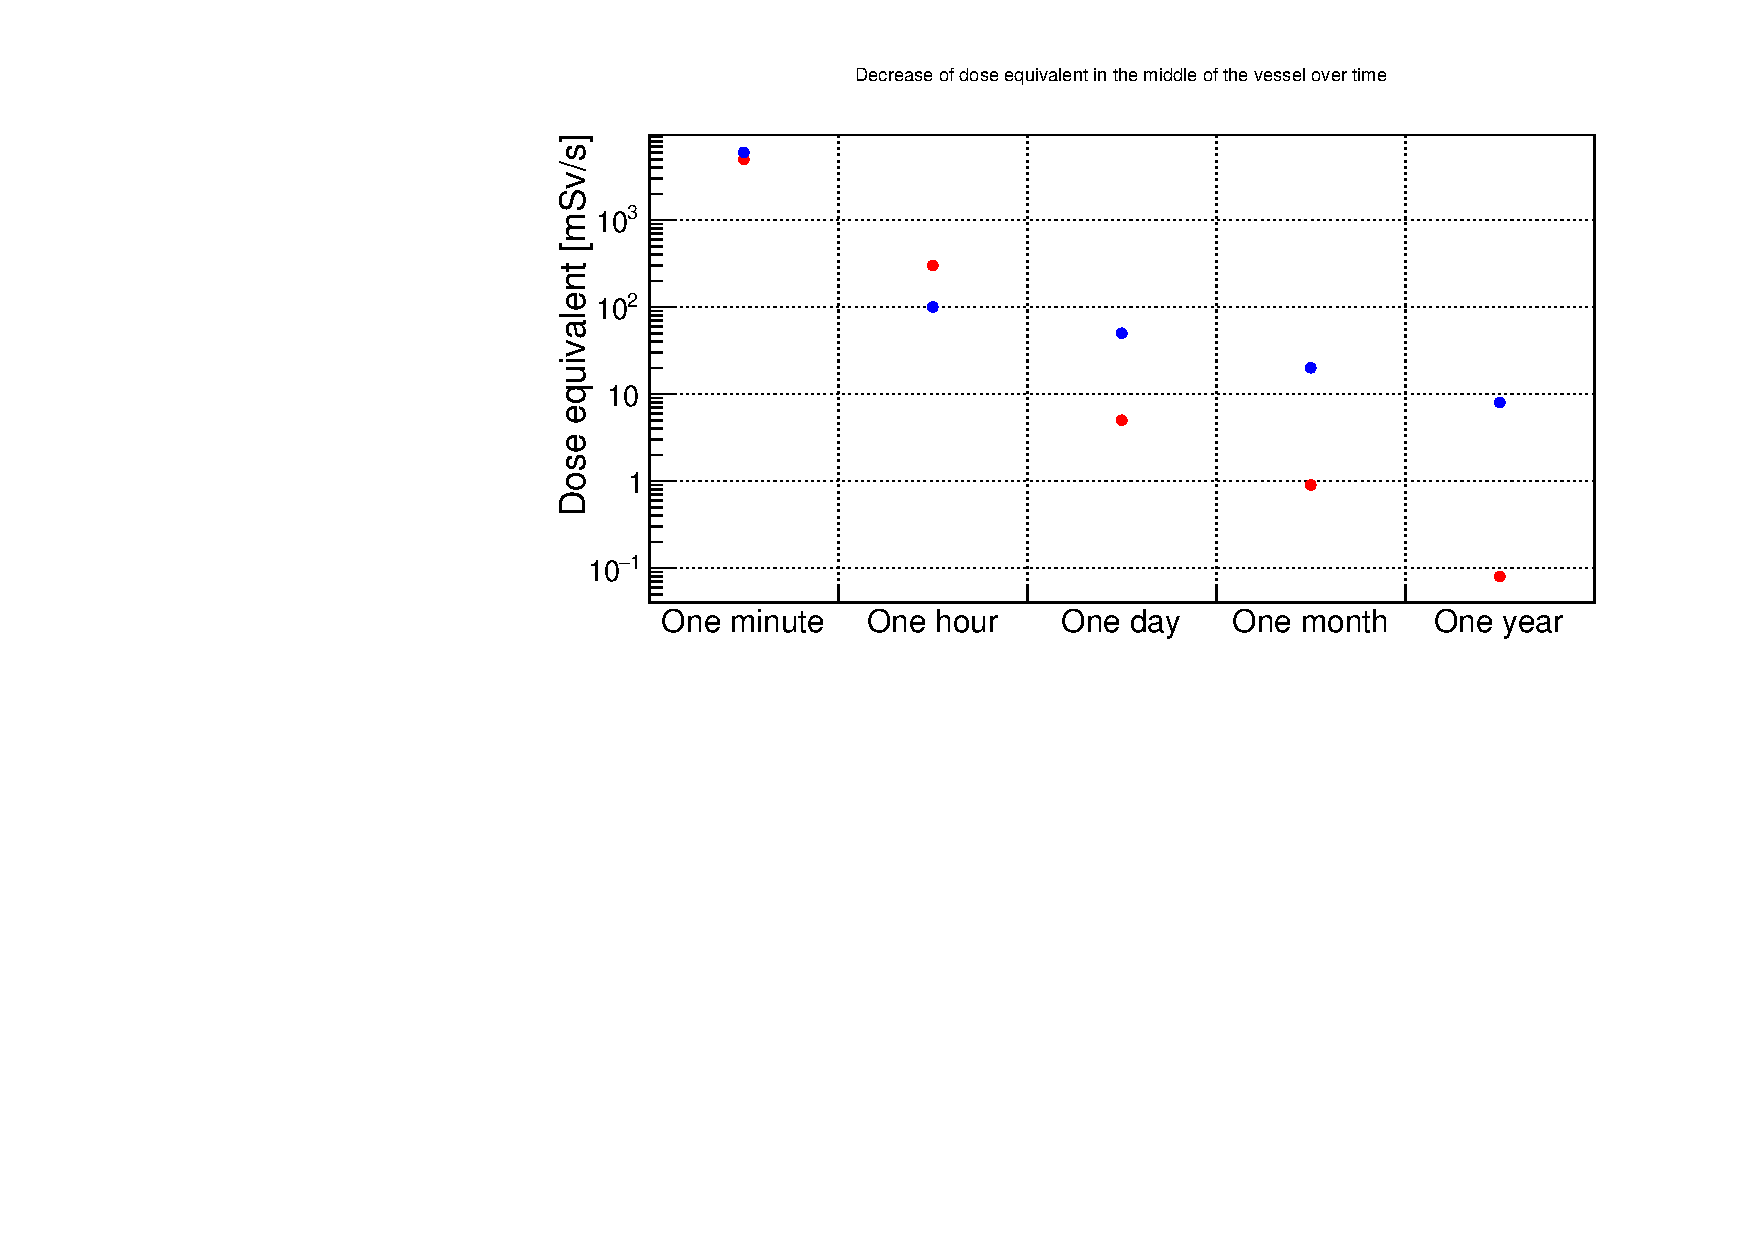
\includegraphics[width=0.7\textwidth]{BeamDump_figures/DoseEQ_Time_Comparison.pdf}
\end{center}
\textbf{After one year}, the dose rate drops to \\\textbf{$\sim$ 0.1\,mSv/s} for \textcolor{Red}{Design 1} and to \textbf{$\sim$ 10\,mSv/s} for \textcolor{Blue}{Design 2}.
\end{frame}

\subsection{Summary and Outlook}
\begin{frame}{Conclusion}
 \flukalogo
 Water beam dump designs:
 \begin{itemize}
  \item The simulations of the two water beam dump designs by B. Smith show \textbf{comparable results}.
  \item The dose rate of the beam dump surrounding is still after one year in the order of \textbf{0.1-1\,mSv/s}.
  \item \textbf{Design 2} seems to be \textbf{more elaborated regarding the water cooling flow system}.
  This leads to \textbf{larger spreads in the energy deposition} due to the high water pressure sections.
 \end{itemize}
 \visible<2->{
 \vspace*{0.2cm}
 FOR FUN:
 \begin{itemize}
  \item Gas dump filled with Nitrogen
  \item Beam dump Design 1 filled with liquid Nitrogen
 \end{itemize}
  }
\end{frame}
\begin{frame}{For Fun: Nitrogen Gas Dump}
 \flukalogo
  \begin{itemize}
  \item Gas dump ($\sim$ 1\,km long) filled with Nitrogen
  \item Adopting ideas from dump design studies for TESLA done at DESY.
  \item Copper walls with a thickness of $\sim$\,60\,cm
 \end{itemize}
 \includegraphics[width=0.5\textwidth]{Other_BeamDumps/Gas_dump/Energy.png}\hfill
 \includegraphics[width=0.5\textwidth]{Other_BeamDumps/Gas_dump/Dose_eq_1year_zoom.png}
\end{frame}
\begin{frame}{For Fun: Design 1 with liquid Nitrogen}
 \flukalogo
  \begin{itemize}
  \item Design 1 (as shown above) filled with liquid Nitrogen
  \item Everything else as before
 \end{itemize}
 \includegraphics[width=0.5\textwidth]{Other_BeamDumps/Liquid_Nitrogen_Dump/Energy.png}\hfill
 \includegraphics[width=0.5\textwidth]{Other_BeamDumps/Liquid_Nitrogen_Dump/Dose_eq_1year.png}
\end{frame}

%---------------------------------------------------------------------------------

\section*{The end}
{
\usebackgroundtemplate{
 \tikz\node[opacity=0.1]{\includegraphics[width=\paperwidth,resolution=200]{figures/ilc-Comic.png}};
 % \tikz\node[opacity=0.2]{\centering\includegraphics[height=\paperheight]{figures/Iwatecomics.jpg}};
 }
\begin{frame}
\ilclogo
\begin{center}
\textcolor{RubineRed}{
	\LARGE Thanks!\\
}
\end{center}
\vspace*{0.5cm}
I am close to handing in my Ph.D. thesis.\\
Detailed explanations of all my studies will be given in my thesis, as well as in SiD confluence pages.\\
Simulation files are already or will be made available to everyone on the grid (/ilc/user/a/aschuetz).
\end{frame}
}

\section*{References}
\begin{thebibliography}{9}
\setbeamertemplate{bibliography item}[text]
\begin{frame}{References for the BDS muon study}
\tiny
\bibitem{MUCARLO_talk}  \emph{ECFA 2016: Talk by Glen White about the MUCARLO simulation of the muons from the muon spoilers}. \url{https://agenda.linearcollider.org/event/7014/contributions/34689/attachments/30076/44961/ILC_muons.pptx}
\bibitem{Jonas_talk}  \emph{DESY summer student program: Talk by Jonas Glomitza (RWTH Aachen) about ``The Impacts of the Muon Spoiler Background on the ILC Detector Performance'', 08. September 2016}. \url{https://indico.desy.de/getFile.py/access?contribId=9&resId=0&materialId=slides&confId=15972}
\bibitem{Suppression}  \emph{FERMILAB-CONF-07-276-AD: ``Suppression of Muon Backgrounds generated in the ILC Beam Delivery System'', Drozhdin et.al, 2007}. \url{https://inspirehep.net/record/771808/files/fermilab-conf-07-276.pdf}
\bibitem{MUCARLO}  \emph{``Calculation of Muon Background in Electron Accelerators using the Monte Carlo Computer Program MUCARLO'', Rokni et.al}. \url{http://www.slac.stanford.edu/cgi-wrap/getdoc/slac-pub-7054.pdf}
\bibitem{MuonBackground_1TeV}  \emph{SLAC-PUB-6385: ``Muon Background in a 1.0-TeV Linear Collider'', L.P. Keller, 1993}. \url{http://www.slac.stanford.edu/pubs/slacpubs/6250/slac-pub-6385.pdf}
\bibitem{MuonBackground_0.5TeV}  \emph{SLAC-PUB-5533: ``Calculation of Muon Background in a 0.5 TeV Linear Collider'', L.P. Keller, 1991}. \url{http://www.slac.stanford.edu/cgi-wrap/getdoc/slac-pub-5533.pdf}
\end{frame}
\begin{frame}{References for the FLUKA study}
\tiny
\bibitem{Smith} B. Smith (Rutherford Lab), \emph{Design drawings 0-TB-0067-300-00-A, 0-TB-0067-210-00-A, 0-TB-0067-404-00-A}, Dec. 2006 - Jan. 2007
\bibitem{Smith_Report} B. Smith (CCLRC Technology Department), \emph{18\,MW Water Beam Dump Concept}, Report 088-D-006-01, Jan. 2007
\bibitem{SLAC_FLUKA} S. Darbha, \emph{Simulation of Neutron Backgrounds from the ILC Extraction Line Beam Dump}, SLAC-TN-07-013, Aug. 2007
\bibitem{NIM_paper} P. Satyamurthy, et al., \emph{Design of an 18\,MW vortex flow water beam dump for 500\,GeV electrons/positrons of an international linear collider}, NIM A 679 (2012) 67-81
\bibitem{CLIC_dump} A. Mereghetti, et al., \emph{FLUKA and Thermo-Mechanical Studies for the CLIC Main Dump}, CLIC-Note-876, Mach 2011
\bibitem{Concrete} K. Okuno, et al., \emph{Application of neutron shield concrete to neutron scattering instrument TAIKAN in J-PARC}, Progress in Nuclear Science and Technology, Vol. 4, pp 619-622, 2014
\end{frame}
\begin{frame}{References for the Pair background study}
\tiny
\bibitem{TDR1} T. Behnke, et al., \emph{The International Linear Collider - Technical Design Report, Volume 1}, 2013.
\end{frame}
\end{thebibliography}

%--------------------------------------------------------------------------------
\section{Backup}
\appendix

\begin{frame}
\begin{center}
\LARGE Additional Material
\end{center}
  \tableofcontents
\end{frame}

\section{ILC}

\subsection{The ILC beam parameters}
\begin{frame}{ILC baseline parameters}
\ilclogo
\begin{center}
	\includegraphics[width=\textwidth]{figures/ILCTDR-VOLUME_3-PART_II_ILCparameters.pdf}
\end{center}
\end{frame}
\begin{frame}{ILC parameters for the different upgrade stages}
\ilclogo
\begin{center}
	\includegraphics[width=0.8\textwidth]{figures/ILCTDR-VOLUME_3-PART_II_ILCparametersUpgrades.pdf}
\end{center}
\end{frame}

\section{BDS muons}
\subsection{Analysis - Spatial distributions}
\begin{frame}{Explanation of spatial distributions}
\sidlogo
 \begin{center}
\includegraphics[height=0.85\textheight]{muons_figures/Explanation_Spatial_distribution_NEW.pdf}
\end{center}
\end{frame}

\subsection{Analysis - Energy distributions}
\begin{frame}{Energy distribution of muons}
\sidlogo
  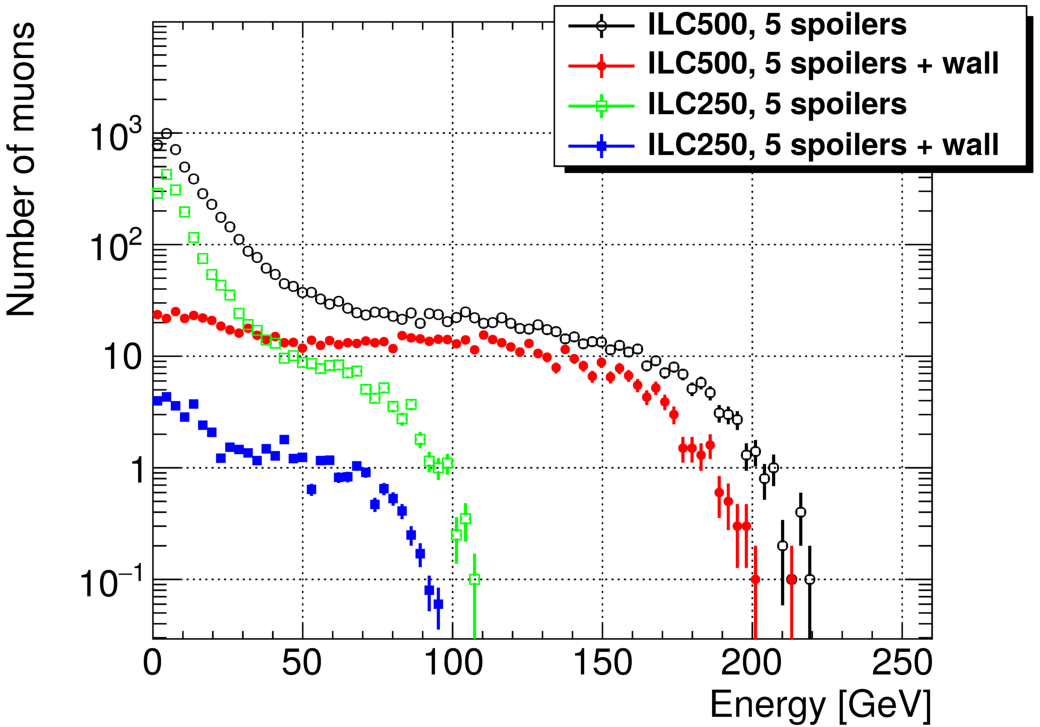
\includegraphics[width=\textwidth]{muons_figures/figures/Energy_Comparison_ILC500vsILC250.pdf}

In the 'Spoiler + Wall' case, the lower energy muons are either stopped or deflected by the magnetized wall.
\end{frame}

\subsection{Analysis - SiD hit distribution}
\begin{frame}{Explanation of hit number distribution -\\ \small Spatial distribution in the MuonEndcaps}
\sidlogo
 \begin{center}
\includegraphics[height=0.78\textheight]{muons_figures/Explanation_Hits_Subdetectors.pdf}
\end{center}
\end{frame}

\subsection{Analysis - SiD Occupancy}
\begin{frame}{Occupancy plots - \small SiTrackerEndcap}
\sidlogo
Low energy muon (order of MeV) is deflected in the magnetic solenoid field, and hits the active layer several times.
 \begin{center}
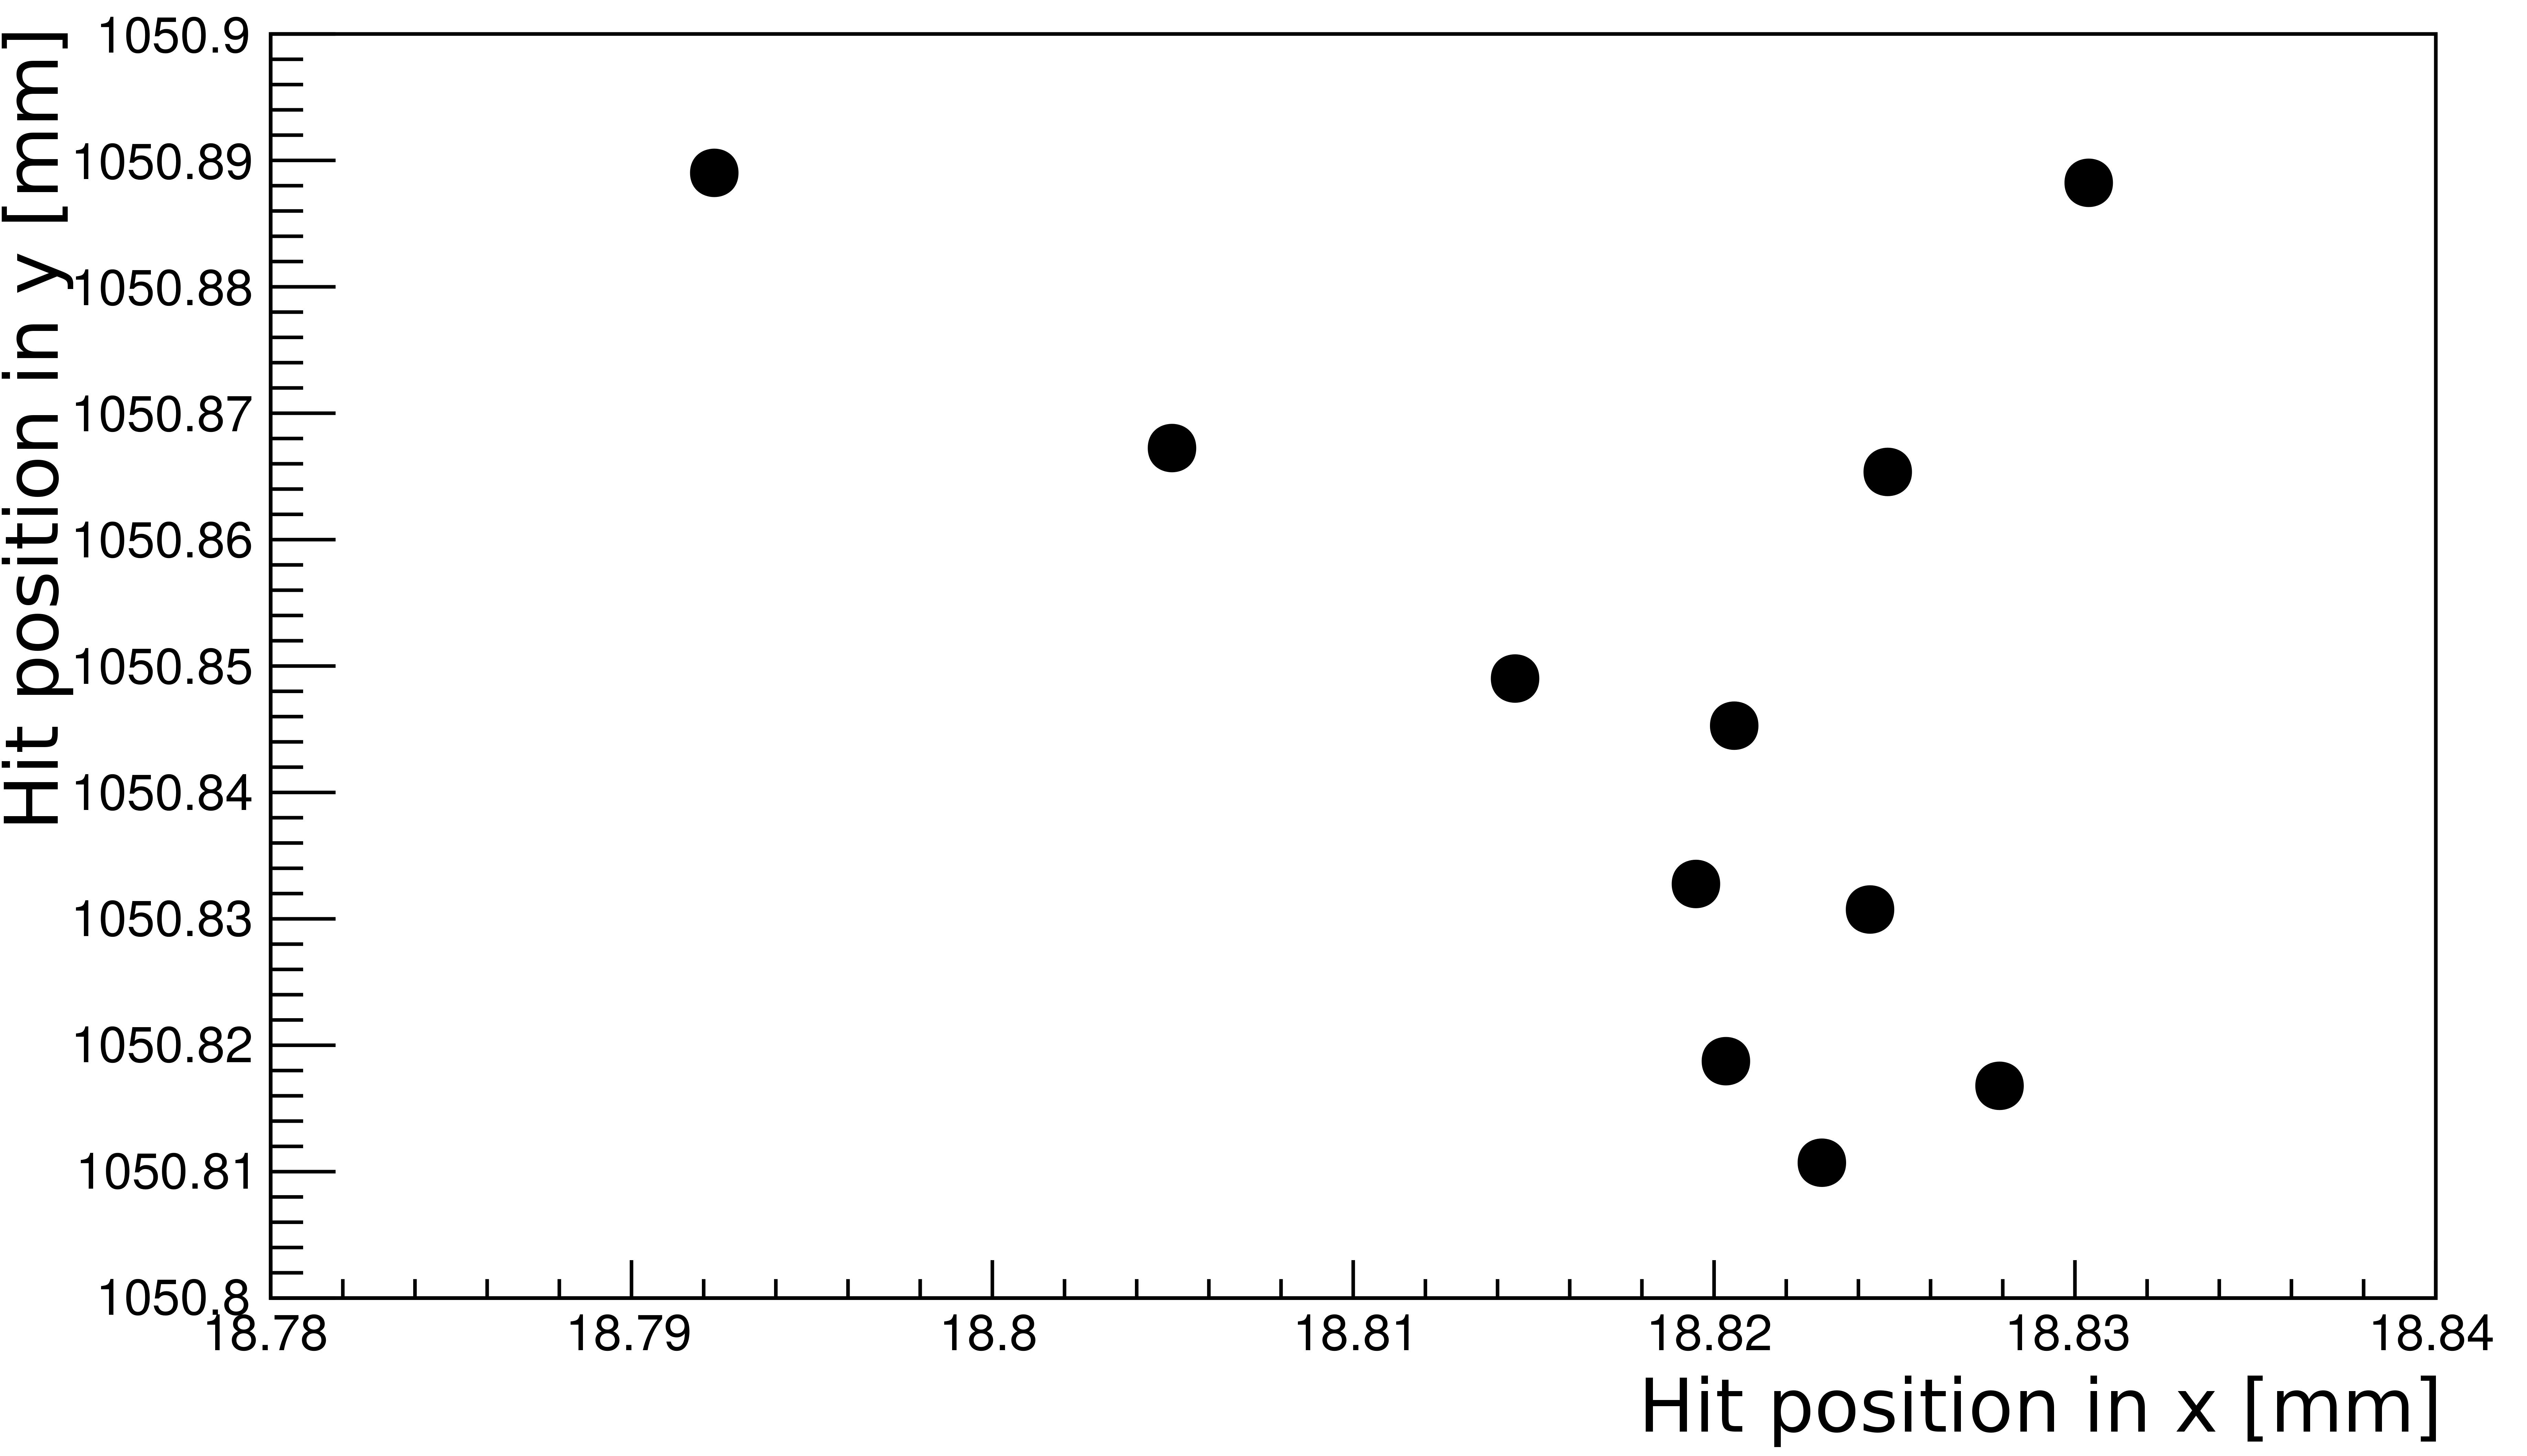
\includegraphics[height=0.65\textheight]{LoopInACell.pdf}
\end{center}
\end{frame}


\subsection{Analysis - Time distributions}

\begin{frame}{Hit Time distribution}
\sidlogo
 \begin{center}
\includegraphics[height=0.65\textheight]{muons_figures/figures/HitTime_Comparison_ILC500vsILC250.pdf}
\end{center}
Muons are first hitting the MuonEndcaps as the most outer subdetector.
\end{frame}

\section{FLUKA simulation}

\subsection{Particle Fluxes}
\begin{frame}{Electron and Photon fluxes from one bunch}
\begin{center}
Design 1 \hspace*{1.4cm} Electrons \hfill Photons \hspace*{3.1cm} \\
 \includegraphics[width=0.37\textwidth]{BeamDump_figures/Electron_flux_xz_Design1.pdf}
  \includegraphics[width=0.37\textwidth]{BeamDump_figures/Photon_flux_xz_Design1.pdf}\\
Design 2 \hspace*{1.4cm} Electrons \hfill Photons \hspace*{3.1cm} \\ 
\includegraphics[width=0.37\textwidth]{BeamDump_figures/Electron_flux_xz_Design2.pdf}
  \includegraphics[width=0.37\textwidth]{BeamDump_figures/Photon_flux_xz_Design2.pdf}
\end{center}
\end{frame}
\begin{frame}{Proton fluxes}
\begin{center}
\hspace*{2cm} Design 1 \hfill Design 2 \hspace*{2cm} \\
  \includegraphics[width=0.52\textwidth]{BeamDump_figures/Proton_flux_xz_Design1.pdf}
    \includegraphics[width=0.52\textwidth]{BeamDump_figures/Proton_flux_xz_Design2.pdf}
\end{center}
\end{frame}
\begin{frame}{Neutron fluxes from one bunch: \textbf{Design 1}}
\begin{columns}
 \begin{column}{0.5\textwidth}
    \includegraphics[width=\textwidth]{BeamDump_figures/Neutron_flux_xz_Design1.pdf}
 \end{column}
 \begin{column}{0.5\textwidth}
  The neutrons spread more in the positive x and y-direction. Within the tank, the neutrons are mainly produced in the water vortex system. When the beam is stopped by the copper plates, the neutron production rate decreases.
 \end{column}
\end{columns}
\hspace*{1cm} x-direction \hfill y-direction \hfill z-direction \hspace*{1cm} \\
  \includegraphics[width=0.31\textwidth]{BeamDump_figures/Neutron_flux_1DMax_x_Design1.pdf}\hfill
  \includegraphics[width=0.31\textwidth]{BeamDump_figures/Neutron_flux_1DMax_y_Design1.pdf}\hfill
  \includegraphics[width=0.31\textwidth]{BeamDump_figures/Neutron_flux_1DMax_z_Design1_withLabels.pdf}
\end{frame}
\begin{frame}{Neutron fluxes from one bunch: \textbf{Design 2}}
\begin{columns}
 \begin{column}{0.5\textwidth}
    \includegraphics[width=\textwidth]{BeamDump_figures/Neutron_flux_xz_Design2.pdf}
 \end{column}
 \begin{column}{0.5\textwidth}
  The neutrons again spread more in the positive x and y-direction. Within the tank, the point of highest neutron production is the high pressure water system. The production rate again decreases with the beam being stopped by the copper plates.
 \end{column}
\end{columns}
\hspace*{1cm} x-direction \hfill y-direction \hfill z-direction \hspace*{1cm} \\
  \includegraphics[width=0.31\textwidth]{BeamDump_figures/Neutron_flux_1DMax_x_Design2.pdf}\hfill
  \includegraphics[width=0.31\textwidth]{BeamDump_figures/Neutron_flux_1DMax_y_Design2.pdf}\hfill
  \includegraphics[width=0.31\textwidth]{BeamDump_figures/Neutron_flux_1DMax_z_Design2_withLabels.pdf}
\end{frame}

\end{document}
